%%%%%%%%%%%%%%%%%%%%%%%%%%%%%%%%%%%%%%%%%%%%%%%%%%%%%%%%%%%%%%%%%%%%%%%%%%%%
%
%  ludwig.tex
%
%  Long-hand documentation for Ludwig. This file is main document
%  with style only. Content is in sections.tex
%
%  $Id$
%
%  Edinburgh Soft Matter and Statistical Physics Group and
%  Edinburgh Parallel Computing Centre
%
%  Kevin Stratford (kevin@epcc.ed.ac.uk)
%  (c) 2008 The University of Edinburgh
%
%%%%%%%%%%%%%%%%%%%%%%%%%%%%%%%%%%%%%%%%%%%%%%%%%%%%%%%%%%%%%%%%%%%%%%%%%%%%

\documentclass[11pt,twoside]{article}

\usepackage{amsmath}
\usepackage{moreverb}
\usepackage{lscape}
\usepackage{epic}

\setlength{\hoffset}{-1in}
\setlength{\voffset}{-1in}

\setlength{\topmargin}{2cm}
\setlength{\evensidemargin}{3.1cm}
\setlength{\oddsidemargin}{3.1cm}

\setlength{\textwidth}{14.8cm}
\setlength{\textheight}{23cm}

\setlength{\parindent}{0pt}
\setlength{\parskip}{\smallskipamount}


\newcommand{\inputkey}[1]{\framebox{\textbf{\texttt{#1}}}}
\begin{document}

\setcounter{page}{1}

\tableofcontents

\newpage

\setcounter{page}{1}

%%%%%%%%%%%%%%%%%%%%%%%%%%%%%%%%%%%%%%%%%%%%%%%%%%%%%%%%%%%%%%%%%%%%%%%%%%%%%
%
%  user.tex
%
%  The 'user' section which holds an overview, and discusses
%  compilation and running.
%
%  $Id$
%
%  Edinburgh Soft Matter and Statistical Physics Group and
%  Edinburgh Parallel Computing Centre
%
%  Kevin Stratford (kevin@epcc.ed.ac.uk)
%  (c) 2010 The University of Edinburgh
%
%%%%%%%%%%%%%%%%%%%%%%%%%%%%%%%%%%%%%%%%%%%%%%%%%%%%%%%%%%%%%%%%%%%%%%%%%%%%%

\section{Introduction}

\subsection{Overview}

We aim to provide a robust and portable code, written in C, which
can be used to perform serial and scalable parallel simulations of
complex fluid systems based around hydrodynamics via the Lattice
Boltzmann method. Complex fluids are introduced via a free energy,
of which a number of different examples are available. The preferred
method of dealing with the corresponding order parameter equations
is now by using finite difference. However, for the case of a binary
fluid, the `full LB' approach, using two distributions, is retained
as an option for the time being.

\subsection{Availability}

Under the auspices of the CCPs (Collaborative Computational Projects),
and in particular CCP5, we have a CCPForge project account at

\texttt{http://ccpforge.cse.rl.ac.uk/}

This provides controlled access to known persons and uses version
control via SVN, and includes bug
tracking, and so on. The CCPForge SVN is not available to the public
at the present time. You need to create an account at CCPForge, and
let me or Juho know the username so you can be added to the access list.

To download the entire code, you need
\begin{verbatim}
svn checkout --username <user> http://ccpforge.cse.rl.ac.uk/svn/ludwig
\end{verbatim}
where \texttt{<user>} is replaced by your CCPForge user name.
Note that this will download all the existing tags and branches
into a new directory named \texttt{ludwig}, as well as the main code!
On success, you should see three directories
\begin{verbatim}
$ ls ludwig
branches  tags      trunk
\end{verbatim}
The main code is in the \texttt{trunk} subdirectory. This documentation is
found in the file \texttt{trunk/htdocs/ludwig.tex}, unit tests are in
the directory \texttt{trunk/tests}, and the utilities are in
\texttt{trunk/util}, and so on.

If you do not want all the tags and branches (which take up a certain amount
of space), you can specify that you
want only the trunk, e.g.,
\begin{verbatim}
svn co --username <user> http://ccpforge.cse.rl.ac.uk/svn/ludwig/trunk
\end{verbatim}
in which case you will get a new directory called \texttt{trunk} containing
the source files. All the instructions below refer to paths relative to
this trunk directory.

If you have problems, it may be worth while looking at the issue
tracker on the project web page. It would be useful if all issues
could be reported via this mechanism. If you e-mail me, I will just
insert your e-mail into the issue tracker!

\subsection{Compilation}

Locate your local C compiler. The following example uses \texttt{gcc}
in serial, and \texttt{mpicc} in parallel. For MPI in particular,
local details may vary.

The other thing required by the Makefile is the utility
\texttt{svnversion}, which allows the compile-time SVN version number to
be included in the executable (and hence the output of the program). This
is useful to remember which version you were using when looking at
results at a later date. If
\texttt{svnversion} is not available (and it
should be if you have downloaded the code via SVN), you may get an
error message, but the code should still compile.

\subsubsection{Serial}

First, compile the MPI stub library in the \texttt{mpi\_s}
directory. Do this by editing the Makefile, and checking the compiler
is appropriate. You should be able to build the library and run the
tests using, e.g.,:

\begin{verbatim}
$ make libc
gcc -Wall -I.  -c mpi_serial.c
ar -cru libmpi.a mpi_serial.o
$ make testc
gcc -Wall   mpi_tests.c -L. -lmpi
./a.out
Running mpi_s tests...
Finished mpi_s tests ok.
\end{verbatim}

Now compile the main code in the \texttt{src} directory. Again
edit the Makefile to check the compiler. At this stage, you also
need to choose the LB model using exactly one of the preprocessor
options for D2Q9 (fluid only problems), D3Q15, or D3Q19. Now type,
e.g., using D3Q19:

\begin{verbatim}
$ make serial
gcc  -D SVN_REVISION='"'`svnversion`'"' -c svn.c
gcc  -D_D3Q19_ -O3 -Wall -I. -I../mpi_s -c d2q9.c
gcc  -D_D3Q19_ -O3 -Wall -I. -I../mpi_s -c d3q15.c
gcc  -D_D3Q19_ -O3 -Wall -I. -I../mpi_s -c d3q19.c
gcc  -D_D3Q19_ -O3 -Wall -I. -I../mpi_s -c model.c
...
\end{verbatim}

This should provide an executable \texttt{Ludwig.exe} which is linked
against the MPI stub library.

\subsubsection{Parallel}

Here, you do not need to compile the stub library. Simply compile
the main code with, e.g.,:
\begin{verbatim}
$ make mpi
mpicc -D_D3Q19_ -O3 -Wall -I. -c d2q9.c
mpicc -D_D3Q19_ -O3 -Wall -I. -c d3q15.c
mpicc -D_D3Q19_ -O3 -Wall -I. -c d3q19.c
mpicc -D_D3Q19_ -O3 -Wall -I. -c model.c
...
\end{verbatim}

Invoke the executable with the MPI launcher in the usual way for your
system, e.g., \texttt{mpirun -np 8 ./Ludwig.exe} for 8 processors,
and so on.

\subsubsection{ANSI C}

The code is ANSI C (1989), with the single exception of calls to the
library function \texttt{erfc()} in the Ewald sum code. This
can sometimes cause a problem, which can usually be solved with
a compiler-specific work-around.

\subsubsection{C assertions}

The code makes quite a lot of use of standard C assertions, which
are useful to prevent errors. They do result in a considerably
slower execution in some instances, so production runs should
switch off the assertions with the standard \texttt{NDEBUG}
preprocessor flag.


\section{User Input}

The executable will look for an input file at run time.
By default, this file is named \texttt{input} and should be in the
current working directory. The alternative is to specify the name
of the file explicitly on the command line:
\begin{verbatim}
$ ./Ludwig.exe input_file
\end{verbatim}
A reference input file \texttt{input.ref} is provided as a template.

The contents of the input file are made up of \textit{key value}
pairs with control the run-time behaviour. Blank lines and lines
begining with \# are ignored as comments. The following describes
the effect of various keys. Most keys have a default value which
will be used by the code if the corresponding key is not present
(or commented out) in the input file.

\subsection{Setting up the input}

Decide what free energy you want and check the relevant sections
of this dcoumentation. If you want a simple fluid only, the free
energy should be set to \texttt{none}.

You should set at least the basic fluid parameters, the system
size, and number of steps to be run.

\textbf{IMPORTANT:} Although many incompatible choices of input
parameters are trapped at run time, you must be careful in how
the input file is set out. If you mistakenly set or unset some
options in the input, erroneous results will surely result...


\subsection{Basic run parameters}

\inputkey{N\_cycles}

The number of lattice Boltzmann time steps to execute. Default
value: 0.

\inputkey{N\_start}

By default the code will start from time step $t = 0$. If you 
wish to restart from a previously saved configuration, set
the appropriate value for \texttt{N\_start}. The code will
execute \texttt{N\_cycles} steps starting from this point.

\inputkey{size}

Controls the number of lattice points in the $(x, y, z)$ directions,
respectively. Default value: 64\_64\_64. If a two-dimensional system
is required, the $z$-direction can be set to 1.

\inputkey{grid}

In parallel, this sets the processor Cartesian decomposition, i.e.,
the number of processors in each dimension of the Cartesian communicator.
The default value may be implementation dependent as it is that returned
by \texttt{MPI\_Dims\_create()}. For
example:
\begin{verbatim}
size 64_64_64
grid 4_2_1
\end{verbatim}
gives a total (physical) system size of 64 lattice sites in each
direction, decomposed across 4 processors in the x-direction, 2 in
the y-direction and 1 (no decomposition) in the z-direction. The
total number of processors must therefore be 8. The local domain
size per processor is then 16x32x64.


\subsection{Fluid properties}

\inputkey{free\_energy}

This sets the free energy in use, and hence has many consequences.
The default value is \texttt{none}, i.e., use a simple fluid only.
The available choices are for symmetric binary fluids, Brazovskii
smectics, polar active gels, and liquid crystals. The surfactant
model is currently being rebuilt.

\inputkey{viscosity}

Sets the LB fluid shear viscosity $\eta$ (and related relaxation time).
Safe values are roughly $0.2 > \eta > 0.0001 $. Default value is 1/6
(i.e., relaxation time equal to unity).

\inputkey{viscosity\_bulk}

Sets the LB bulk viscosity $\zeta$ (and related relaxation time).
This can be useful if you are concerned with incompressiblity
violations, in which case $\zeta >> \eta$ can be useful. The
default value is $\zeta = \eta$.

\inputkey{isothermal\_fluctuations}

This switches on the fluctuationing hydrodynamics. Default is off.

\inputkey{temperature}

The LB 'temperature' using fluctuating hydrodynamics. Safe values
are $0.0001 > kT > 0$. 

\inputkey{ghost\_modes}

Allows you to switch the ghost modes off in the collision stage.
Default is on.


\subsection{Symmetric binary fluid}

\inputkey{free\_energy symmetric}

The following applies for the binary fluid problem with
compositional order parameter $\phi$ and free energy
(excluding the term in the density $\rho$):
\begin{equation}
 F[\phi] = 
\int dr \left(
{\textstyle \frac{1}{2}}A\phi^2
+ {\textstyle \frac{1}{4}}B\phi^4
+ {\textstyle \frac{1}{2}}\kappa (\mathbf{\nabla}\phi)^2 \right).
\end{equation}

This is described in some detail
by Kendon et al \cite{viv}. The first two terms represent the bulk
contribution, whereas the term in $\kappa$ penalises curvature in
the interface.

\inputkey{A} The parameter $A$. Note $A < 0$.

\inputkey{B} The parameter $B$. Note $B = -A$ for common usage,
although this is not enforced.

\inputkey{K} The parameter $\kappa$, which is positive.

The order parameter evolution is determined by a Cahn-Hilliard equation
with mobility set by

\inputkey{mobility} Sets mobility $M$ (uniform in space).

The following parameters control the initialisation of the order
parameter.

\inputkey{phi\_initialisation}

Determines how the compositional order parameter is initialised
at the start of the run. If set to \texttt{spinodal} the value
is set to $\phi_0$ as set above plus or minus a random noise, the
magnitude of which is set by the value of the \texttt{noise} key.
If set to \texttt{block} a one-dimensional profile is set up in
the $z$-direction representing two blocks of fluid with
$\phi = \pm 1$. The two interfaces are set at $z = L_z/4$ and
$z = 3L_z/4$ with the equilibrium $\tanh(z/\xi_0)$ profile having 
appropriate width. The $\phi = -1$ section is in the middle.

\inputkey{phi0}

The mean compositional order parameter roughly $-0.5 < \phi_0 < 0.5$.
The default value is zero, i.e., a symmetric 50:50 mixture by volume.

\inputkey{noise}

The magnitude of the initial fluctuations in $\phi$ used to
initiate spinodal decomposition.

\subsubsection{Binary fluid using two distributions}

\inputkey{symmetric\_lb}

This is the special case where the composition is represented
by a second LB distribution, and an appropriate lattice kinetic
equation approximating the Cahn-Hilliard equation is solved.
In this case the above parameters have the same meaning.


\subsection{Brazovskii}

\inputkey{free\_energy brazovskii}

This is similar to the symmetric free energy, but with one extra term
in a higher derivative of $\phi$.
\begin{equation}
 F[\phi] = 
\int dr \left(
{\textstyle \frac{1}{2}}A\phi^2
+ {\textstyle \frac{1}{4}}B\phi^4
+ {\textstyle \frac{1}{2}}\kappa (\mathbf{\nabla}\phi)^2
+ {\textstyle \frac{1}{2}} C (\nabla^2 \phi)^2 \right).
\end{equation}

The parameters now include $C$. For $A<0$, phase separation occurs
with a result depending on $\kappa$: ones get two symmetric phases
for $\kappa >0$ (cf. symmetric) or a lamellar phase for
$\kappa < 0$.

\inputkey{A} Bulk parameter $A < 0$.

\inputkey{B} Bulk parameter $B = -A$.

\inputkey{K} Negative for lamellar phase.

\inputkey{C} Positive.

Other parameters, including the mobility, are set as for the
symmetric free energy (see above).


\subsection{Surfactant in binary fluid}

\inputkey{free\_energy surfactant}

Currently under reconstruction.

This is for use with a two order parameter model the first of
which is the composition, as for the symmetric free energy,
while the second $\psi$ represents surfactant concentration.
The free energy density is made up of a number of terms:

\begin{equation}
{\textstyle \frac{1}{2}}A\phi^2
+ {\textstyle \frac{1}{4}}B\phi^4
+ {\textstyle \frac{1}{2}}\kappa (\mathbf{\nabla}\phi)^2
\end{equation}
is the standard symmetric term related to the composition.
These parameters are represented in the input as

\inputkey{surf\_A}
\inputkey{surf\_B}
\inputkey{surf\_kappa}

\begin{equation}
D \left(\psi \ln\psi + (1 - \psi) \ln(1-\psi)\right)
\end{equation}
represents the energy of surfactant in the bulk phase with surfactant
concentration $0 < \psi < 1$ with a single parameter $D$;
\begin{equation}
-{\textstyle \frac{1}{2}} \epsilon \psi (\mathbf{\nabla} \phi)^2
-{\textstyle \frac{1}{2}} \beta \psi^2  (\mathbf{\nabla} \phi)^2
\end{equation}
where the term in $\epsilon$ represents the energy reduction by
adsorbing surfactant at the interface and the term in $\beta$
provides an additional favourable term modelling the fact that
the molecules like to line up; finally, there is an extra term
\begin{equation}
+{\textstyle \frac{1}{2}} W \psi \phi^2
\end{equation}
which is included to stabilise the interface \cite{theissengompper}.

The corresponding keys for the input file are:

\inputkey{D} is the bulk surfactant contribution parameter

\inputkey{epsilon} is the parameter $\epsilon$

\inputkey{W} is the parameter $W$

\inputkey{beta} is the value of the parameter $\beta$.

\inputkey{phi\_b} the initial, uniform, background surfactant
concentration $\psi_b$.

\inputkey{mobility\_psi} Sets the (uniform) mobility for the surfactant
as appropriate for the Cahn-Hilliard equation.


\subsection{Polar Active Gel}

\inputkey{free\_energy polar\_active}

This models a polar active gel with vector order parameter $P_\alpha$.
The free energy density is:


The corresponding input parameters are:

\inputkey{polar\_active\_a}

\inputkey{polar\_active\_b}

\inputkey{polar\_active\_k}

\inputkey{polar\_active\_klc}

\inputkey{polar\_active\_zeta}

\inputkey{polar\_active\_lambda}

\inputkey{leslie\_ericksen\_gamma}

\inputkey{leslie\_ericksen\_swim}


\subsection{Liquid Crystal}

\inputkey{free\_energy lc\_blue\_phase}

Here, we have a tensor order parameter $Q_{\alpha\beta}$.
The free energy density is
\begin{eqnarray}
f = {\textstyle\frac{1}{2}}A_0(1 - \gamma/3)Q^2_{\alpha\beta}
  - {\textstyle\frac{1}{3}}A_0 \gamma
Q_{\alpha\beta}Q_{\beta\delta}Q_{\delta\alpha}
 + {\textstyle\frac{1}{4}}A_0 \gamma (Q^2_{\alpha\beta})^2
\nonumber
\\
+ {\textstyle\frac{1}{2}} \Big(
\kappa_0 (\epsilon_{\alpha\delta\sigma} \partial_\delta Q_{\sigma\beta} +
2q_0 Q_{\alpha\beta})^2 + \kappa_1(\partial_\alpha Q_{\alpha\beta})^2 \Big)
\end{eqnarray}

The corresponding input parameters are:

\inputkey{lc\_a0} The bulk free energy parameter $A_0$

\inputkey{lc\_gamma} The bulk free energy parameter $\gamma$

\inputkey{lc\_q0} The pitch wavenumber $q_0 = 2\pi / p$, where p
is the pitch.

\inputkey{lc\_kappa0} Elastic constant $\kappa_0$ in distortion free energy

\inputkey{lc\_kappa1} Elastic constant $\kappa_1$ in distortion free energy

Note that the code currently enforces the `one elastic constant'
approximation ($\kappa_0 = \kappa_1$), so both these values must
be equal in the input. This constraint may be relaxed in the future.


\inputkey{lc\_Gamma} The rotational diffusion constant appearing in
the Beris Edwards equation (note \texttt{lc\_gamma} and \texttt{lc\_Gamma}
are different).

\inputkey{lc\_xi} Aspect ratio for rod lie molecules appearing in the
stress tensor.

\inputkey{lc\_active\_zeta} Apolar liquid crystal activity constant.

\subsubsection{Initial LC order parameter $Q_{\alpha\beta}$}

\inputkey{lc\_q\_initialisation}

There are a number of useful choices here. The key value
\texttt{twist} initialises a simple cholesteric with the
helical axis in the $z-$direction, whereas the values 
\texttt{cholesteric\_x\_y\_z} provide similar initialisations 
with twist along the other axes.
The values \texttt{o8m} and \texttt{o2} give equilibrim BPI and BPII.
Another, cubic body-centered BP is obtained by the value \texttt{o5}.
Hexagonal BPs are initialised with \texttt{h2d, h3da} and \texttt{h3db}.\\
BPIII emerges from a start configuration of randomly positioned 
and oriented DTCs embedded into an isotropic or cholesteric environment.
This is initialised with the key value \texttt{bp3}, whereas the number
$N$ and radius $R$ of the DTCs and the type of the environment 
$ENV=\{0,1\}$, (0 = isotropic, 1 = cholesteric) is specified 
with the key value \texttt{lc\_init\_bp3} $N\_R\_ENV$. 
Note that calculations can become surprisingly unstable if the 
start configuration consits of too many and too large DTC-regions 
with respect to system size and decomposition.\\
The appropriate choices for the other parameters must be made correspondingly.

An additional \texttt{lc\_q\_init\_amplitude} value sets the
scalar order parameter  `amplitude' in each case. Typical
values are given in the input file. Values which are too large can
equally lead to instability.

\subsubsection{The redshift}

\inputkey{lc\_init\_redshift}

Sets the initial value of the redshift parameter. For example,
for the \texttt{o8m} initialisation, the redshift can be set to 0.83,
and for the \texttt{o2} initialisation, the redshift can be set to 0.91.
The default redshift is unity.

\inputkey{lc\_redshift\_update [0|1]}

Switches on (default is off) the dynamic computation of the redshift
from the order parameter gradient terms in the free energy. The
caluclation is performed at every time step, and override any
initial value specified in the above. It is also robust to restarts.

\subsection{Colloidal particles}

The are a number of important options required for colloids. If
none of these keys are present, no colloids will be used.

\inputkey{colloid\_init}

This determines how the code initialises particles (or not). As stated, the
default is to have no particles (value \texttt{no\_colloids}). There
are two other options at the moment.

There are two options:

\inputkey{colloid\_init    from\_file}

requires a preprepared file of colloid information. To understand
how to create such a file in the correct format,
see the example program \texttt{colloid\_file.c} in the util
directory.

\inputkey{colloid\_init   random}

This may be useful to initialise a limited number of colloids at
low volume fraction. Note that there is no guarantee that the
particles do not overlap, in which case the initialisation will
terminate. The number of particles and their properties
are determined by the value of the keys described below.

\inputkey{colloid\_type}

This controls the the type of particle. Appropriate values are
\texttt{inactive}, giving a standard fully resolved LB colloid;
\texttt{active} switches on the correction to BBL appropriate
for active particles (expecting parameters $b_1$ and $b_2$ to be
set); \texttt{subgrid} gives unresolved particles (radius $< 1$
lattice unit) and no BBL.

If more than one particle is used, all positions are set at random.


\inputkey{colloid\_gravity  0.0\_0.0\_-0.0001}

Sets a body force on each particle. Useful, for example, for
sedimentation. For example, the above gives a constant force in
the negative $z$-direction on each particle.
The code automatically computes the compensating body force on fluid
nodes required to give no net change in the total momentum of the
system at each time step.

\subsubsection{Interactions and the cell list}

In each local domain, colloidal particles are stored in a cell list.
This is a common structure in molecular dynamics-like problems. Here,
it also serves as the basis for parallel communication of colloid
information, so there are a number of constraints which it is important
to understand. In particular, parallel communication imposes the
constraint that there be at least 2 cells in the local domain in
each coordinate direction.

The size of the cells is computed automatically by the code based on
the local domain size, particle size, and the cut-off distance of any
pairwise interactions that are relevant. This will usually mean trying
to maximise the number of cells (to reduce pairwise interaction
calculation). The user must set the minimum allowable cell width.

\inputkey{colloid\_cell\_min}

This sets the minimum cell list width. This key must be set and there
must be at least two cells per processor domain. If the minimum does
not capture the specified interactions, a fatal error will result.
For spherical particles, the minimum width will typically be
$2a_h + h_c$ where $h_c$ is an interaction cut-off distance.


In the case where very large particles are required, it can be useful
to switch of the cell list. This is done via

\inputkey{colloid\_cell\_list\_interactions no}

The constraint in this case is that $2a_h + h_c < L_{local}$, ie.,
there is effectively one cell in each local domain. (In practice,
the constraint is slightly tighter than this if larger halo regions
are in effect.) This option
should not be required in normal circumstances.


\subsubsection{Initialisation from file}

A file containing initial state properties for one or more colloids
can be read at run file. This file must be of the correct from, but
can be ASCII or binary. To help to create such a file, an example
is given in \texttt{./util/colloid\_file.c}. This file will be
read correctly in both serial and in parallel. Colloid positions
should always be in terms of the global coordinates. By default,
the input expected is \texttt{config.cds.init.001-001}.

All colloid output is in serial (ie., a single file is produced)
at the moment. Again, it may be ASCII or binary.

\subsubsection{The colloid state}

The full data structure for the colloid state is defined in
\texttt{src/colloid.h} and the corresponding routines which read
and write the values are in \texttt{src/colloid.c}
(note colloid singular!). Most of the state corresponds clearly
with physical properties, although there are a number of 'structural'
elements which have no physical meaning. These include the
\texttt{rebuild} flag, which instructs the code to reconstruct the
boundary links if necessary, and \texttt{deltaphi} which is involved
in accounting for conserved order parameter in the \texttt{symmetric\_lb}
free energy. Further, not all the elements are relevant is all
circumstances: e.g., the magnetic dipole is only relevant is magnetic
interactions are required, and squirmer parameters are only relevant
to active particles.

Note that it is possible in principle to have magnetic active particles,
in which case the dipole direction (\texttt{s}) and the direction of
motion vector (\texttt{m}) are allowed to be distinct.

\subsubsection{Initialisation at random}

\inputkey{colloid\_random\_no} Sets the total number of particles

\inputkey{colloid\_random\_a0}

\inputkey{colloid\_random\_ah}

\inputkey{colloid\_random\_dh}

The parameter $a_0$ the nominal radius of the particle on the lattice.
This is used to construct the links for BBL. The smallest acceptable LB
particle is $a_0 = 1.25$ (approximately). There are 'magic' values
including 1.25, 2.3, 3.7, 4.77 which minimise discretisation effects.
The hydrodynamic radius of the particles is $a_h$. For all
reasonable applications choose $a_h = a_0$. This is the radius for
all physical purposes. The \texttt{colloid\_random\_dh} parameter
specifies the smallest allowed surface-surface separation if two or
more particles (or walls) are required. This is useful to prevent
very close particles experiencing large and destabilising interactions
at start time.

The other state for the initial colloids can be set uniformly by
means of the keys:

\inputkey{colloid\_random\_v0} initial velocity vector

\inputkey{colloid\_random\_w0} initial angular velocity vector

\inputkey{colloid\_random\_s0} initial spin vector (only relevant in magnetic
field)

The 

\inputkey{colloid\_random\_m0} initial direction of motion vector for active
particles

\inputkey{colloid\_random\_b1} active parameter $b_1$

\inputkey{colloid\_random\_b2} active parameter $b_2$ (should be combined
with the \texttt{active} particle type key as discussed above).

The squirmer parameters specify the surface boundary conditions in
an approach originating with Lighthill \cite{lighthill} and Blake
\cite{blake}. Briefly, $b_1$ sets the propulsion speed
($U = {\frac{2}{3}} b_1$), while $b_2$ sets the
particle stresslet. The ratio $\beta = b_2/b_1$ determines the
mode of the squirmer motion; see \cite{isaac} for further details.


There is one special case. If you want exactly one particle, you may
set its initial position with

\inputkey{colloid\_random\_r0} the initial position vector.

This position must be within the current system, or no particle will
be created.

\subsubsection{Restarting at random!}

Be careful if you are restarting a simulation that used the random
initialisation at $t=0$. You must change to 

\texttt{colloid\_init  from\_file}

to avoid generating a completely new set of random positions
(which will not be consistent with the density and order parameter
fields at the restart time). This is almost certainly not what you
intended!

\subsubsection{Hydrodynamic radius}

There is an important issue to understand about the (nominally)
spherical particles in LB. The input radius $a_0$ is used to
construct the link boundary conditions. However, discretisation
errors in the boundary conditions means that the `real' particle
size may be different. This real radius is the hydrodynamic radius $a_h$.
As a further complication, the hydrodynamic radius can also
be a function of viscosity for a given input radius. Some values
are given in Table~X. This values are computed using a calibration
procedure described by Nguyen and Ladd \cite{nguyen-ladd2002}.

\begin{table}[h]
\begin{center}
\begin{tabular}{|c|c|c|c|}
\hline
$\eta$ & \multicolumn{3}{c|}{$a_0$}\\ \cline{2-4} 
       & 1.25 & 2.30 & 4.77 \\
\hline
1/6  & 1.09 (1.05) & 2.23 (2.20) & 4.76 \\
1/100  & 1.40 (1.34) & 2.50 (2.46) & 5.01 \\
1/1000  & 1.63 & 2.71 & 5.23 \\
\hline
\end{tabular}
\end{center}
\caption{A table of calibrated hydrodynamic radii as a function of input
radius and fluid viscosity $\eta$. These figures are for D3Q19 (and D3Q15
in brackets).}
\end{table}

If a calibration is required for a given radius and viscosity,
use the \texttt{calibration on} key pair in the input file. Some
examples are given in the \texttt{tests/calibration} directory.
An apppropriate
number of time steps must be used to allow the system to get over
the initial transient (we use the momentum diffusion time for the
system $L^2/\eta$) and to allow at least one
particle Stokes time ($a/U$). The input radius and hydrodynamic
radius should be set the same in the input file.

% PENDING Ginzburg d'Humieres correct to ghost mode relaxation times

\subsection{Boundary conditions}

Solid planar boundary walls can be added at the extremities of the
system (i.e., the volume of fluid is exactly that specified by
the \texttt{size} keyword). The wall can be in one, two or all three
coordinate directions, i.e., a 'slab' geometry, and 'duct' geometry
or a 'box' geometry, respectively.

The boundary walls are switched on via the keyword

\inputkey{boundary\_walls}

and with a complementatary specification of the key \texttt{periodicity}.

For example, walls at $x = x_{\min}$  and $x = x_{\max}$  are specified
by

\inputkey{boundary\_walls 1\_0\_0}

\inputkey{periodicity 0\_1\_1}

Both must be present. Note that there are a number of constraints on
valid choices, and the code will stop if there is an invalid choice, or
the two keys above do not match. Common choices are:
\texttt{boundary\_walls 0\_0\_1},
which gives periodic boundaries in the $x-$ and $y-$directions, with
walls at either edge in the $z-$direction; \texttt{0\_1\_1}
gives periodic conditions in the $x-$ direction only, while
\texttt{1\_1\_1} is a fully enclosed box.

In the case of the slab geometry with walls at $z = z_{\min}$ and
$z= z_{\max}$ (only),
two further values are used so that shear may be imparted to the system:

\inputkey{boundary\_speed\_bottom}

\inputkey{boundary\_speed\_top}

These values set the $x-$component of the wall velocity at
$z = z_{\min}$ and $z = z_{\max}$, respectively. Like all
velocities, these values must respect the low Mach number
constraint $u_x < c_s$.

There is a further option for use with the special case in which
top and bottom walls in the $z-direction$ are used to drive a shear
flow (typically with the top speed positive and the bottom speed
negative). The key

\inputkey{boundary\_shear\_init}

may be switched on (set to 1) to provide initialisation of the
LB distributions appropriate for the specified shear rate based
on a linear velocity profile in the $z-$direction. The default
is to initialise the fluid at rest.

\subsubsection{Flat wall lubrication correction}

It is possible to prevent colloids colliding with the flat boundary walls
by adding the correction to the normal component of the lubrication
force. The general form of this correction is
\begin{equation}
\mathbf{F}_{\mathrm{lub}} = -6\pi \eta a_h^2
%({\textstyle \frac{1}{h} - \frac{1}{h_c}})
(1/h - 1/h_c)
\mathbf{u} . \mathbf{r}.
\end{equation}
Here, $h$ is the surface to surface separation, and $h_c$ is the cutoff
distance beyond which the correction is not applied. The relative
velocity (assuming the wall is not moving) and normal separation are
$\mathbf{u}$ and $\mathbf{r}$ respectively.

The cutoff distance can be set from the input via

\inputkey{boundary\_lubrication\_rcnormal 0.1}

where the value is (strictly) set via calibration, cf. the hydrodynamic
radius. In general, the cutoff is between zero and 0.5 lattice spacing,
and can be smaller for larger particles. Because the wall velocity is
fixed, this force correction should cause no stability issues in the
colloid velocity update (provided a colloid's initial position is not
very close to the wall). By default the cutoff $h_c = 0$.

\subsection{Lees-Edwards planes}

\inputkey{N\_LE\_plane}

sets the total number of Lees-Edwards planes. Default is zero.
The placing is as followings. The number of planes $n$ must
divide the lattice size in the $x$-direction to give an integer
$\delta x$. Planes are then placed at $\delta x / 2, 3\delta x/2, \ldots$.

\inputkey{LE\_plane\_vel}

sets the velocity of each plane relative to the lattice. All planes
have the same, constant, velocity.

\inputkey{LE\_init\_profile}

if set to 1, the fluid velocity is initialise to reflect a steady
state shear flow appropriate for the number of planes at the
given velocity. If set to zero, the fluid is initialised with
zero velocity.

Note that when the Lees Edwards boundaries are in place, output
files containing lattice quantities must be `unrolled' to remove
the time-dependent displacement of the planes. This is done using
the extraction utility (see section on parallel I/O).

The code works out the
current displacement of the planes by computing $U_{LE} t$, where
$t$ is the current time step. A shear run should then start from
$t = 0$, otherwise an offset is required.

\inputkey{LE\_time\_offset}

It is often convenient to run an equilibration with no shear, and
then to start an experiment after some number of steps. This
key allows you to offset the start of the Lees-Edwards motion.
It should then take the value of the start time (in time steps)
corresponding to the restart at the end of the equilibration
period. You also need to take this value into account when unrolling
the output.

\subsubsection{Lees-Edwards planes in parallel} 

There are a couple of additional constraints to use the Lees-Edwards
planes in parallel. In particular, the planes cannot fall at a
processor boundary in the $x$-direction. This means you should
arrange an integer number of planes per process in the $x$-direction.
(For example, use one plane per process; this will also ensure the number
of planes
still evenly divides the total system size.)
This will interleave the planes with the processor decomposition.
The $y$-direction and $z$-direction may be decomposed without
further constraint.

Note that this means a simulation with one plane will only work
if there is one process in the $x$ decomposition.

\subsection{Input/Output}

\subsubsection{Serial I/O and standard output}

A variety of information is printed to standard output during the
course of the simulation. This should allow the user to keep track
of basic progress in terms of integrated quantities, total mass,
total momentum and so on. Frequency of output is controlled by

\inputkey{freq\_statistics}

which is an integer. Note that these global statistics require
global communication, and so can affect performance in parallel.
It is recommended that the frequency is kept to a minimum for
large systems (e.g., every 500 or 1000 time steps). This
consideration is true for most types of output (see section
on parallel I/O).

\subsubsection{Configurations}

It may be appropriate to save entire model configurations from
time to time, and certainly when a restart is wanted. For each lattice
quantity, in addition to the data themselves, the program produces a
single meta-data file (ending in
\texttt{.meta}) which is used to describe these data. Colloid
data does not require a meta-data file at the moment.

\inputkey{freq\_config}

This is an integer and sets the frequency of full configuration dumps.
These may be large depending on the size of the system.
Full configurations should consist of the LB distributions,
order parameter (if present) and colloids (if present).


\inputkey{config\_at\_end [yes | no]} 

forces (or switches off) a configuration dump at the end of the run.
The default is to produce a configuration at the end of the run.

\subsubsection{Other lattice quantities}

A number of other lattice-based quantities are available as output.

\inputkey{freq\_measure}

sets the frequency of recording of colloid/order parameter output.
This includes the combined scalar order parameter and director
field output in the case of the liquid crystal free energy.

\inputkey{freq\_phi}

set frequency of order parameter output.

\inputkey{freq\_vel}

set frequency of velocity output. Note that all the hydrodynamic
quantities can be reconstructed from the distribution output, if
available. If only the velocity field is required, this method
allows a considerable saving in storage.

\subsubsection{Colloid I/O}

Colloid I/O is controlled via a series of key value pairs. These are:

\inputkey{colloid\_io\_freq}

gives output at this frequency in time steps. Output is also generated
at configuration steps (and measurement steps at the moment).

\inputkey{colloid\_io\_grid} integer vector

sets the colloid I/O grid. It must be accomodated by the current
choice of \texttt{grid}.

\inputkey{colloid\_io\_format\_input}

One of \texttt{ASCII}, \texttt{ASCII\_SERIAL}, \texttt{BINARY}, or
\texttt{BINARY\_SERIAL}

\inputkey{colloid\_io\_format\_output}

For output, only \texttt{ASCII} or \texttt{BINARY} are available.
 

\subsubsection{I/O format}


\inputkey{vel\_format}

\inputkey{phi\_format}

May be either \texttt{ASCII} or \texttt{BINARY}. Default is \texttt{BINARY}.
Configuration I/O is always in binary. It is recommended to use
binary output for speed and disk space considerations. For a local
sub-domain, the order of the output in the file follows the standard
loop order in the code, i.e., with the $z$-direction running fastest,
then $y$, and with $x$ running slowest. For vector quantities
(anything with more components than a scalar), the vector at each
lattice site appears contiguously.

\subsubsection{Parallel I/O}

In serial, each output quantity appears in one file (\texttt{phi-}
and so on). In parallel, this is also the case by default. However,
this does not scale, owing to the fact that each process has to
write to the same file in turn (ie., in serial). The solution is
to make the I/O parallel. This is done by splitting the domain into
different ``I/O grids'' each of which writes to a separate file.

The default I/O grid can be set using, e.g.,

\inputkey{default\_io\_grid 2\_2\_2}

meaning that the domain is decomposed into a 2x2x2 Cartesian
decomposition for I/O purposes. This will give rise to a total
of 8 files per I/O event with extensions \texttt{.008-001} to
\texttt{.008-008}. These files must be recombined if analysis
is required. However, restarting can be performed with the
parallel files.

Individual lattice quantities can use separate I/O grids. This
may be particularly useful for the distribution data, which are
much larger than the other lattice quantities. This means a
finer decomposition may be appropriate. Clearly, the size of the
I/O decomposition cannot exceed the processor decomposition.
See the advice in section \ref{section-advice} for guidelines.



\subsection{Miscellaneous}

\inputkey{random\_seed}

sets the random number generator seed.

\subsection{Dealing with the Parallel I/O files}

When running in parallel, output of lattice-based (and particle)
quantities takes place in parallel. As a consequence, the order
of the output in the files is not in the same order as would be
the case in serial. This means the parallel output must be
manipulated into the correct order before any analysis.

Parallel I/O subdivides the processors into one or more groups,
each of which write data to a separate file. Information on the
content of each of these files is contained in `meta-data' file
for each quantity, which are produced automatically at the start
of each run. The files are called, e.g., \texttt{phi.001-001.meta}.
If there are 8 I/O groups, the files will be named \texttt{008-001}
to \texttt{008-008} for the different groups.

The actual data is stored for each relevant time step as, e.g.,
\texttt{phi-000100.001-001} where the extension refers to the
I/O. To recombined a single, or multiple, data files into a
single file in the correct order, a utility program
\texttt{extract.c} is provided.

The executable takes two arguments, e.g.,

\inputkey{./extract phi.001-001.meta phi-000100.001-001}

where  the first is the first meta-data file in the relevant series,
and the second is the first data file for the relevant time step. The
program will combine the relevant quantities in the correct order
and produce a single new file \texttt{phi-000100} (in the above case).

\subsection{Restarting}

When restarting in parallel, the processor decomposition must be
preserved. An attempt to change the processor decomposition will
cause the configuration files to be read in the incorrect order,
and results will be wrong.

\section{Parallel Performance}

\subsection{General Comments}

The basic LB calculation should scale well in parallel, that is,
the time taken for fixed problem size will decrease linearly
with the number of MPI processes (strong scaling), or a larger
problem can be run on a proportionally larger number processes
in the same time (weak scaling). To ensure performance is retained
in parallel, it is useful to understand some basic considerations.
Some of these are discussed below.

\textit{Ludwig} has been run successfully on up to 131,072 MPI
tasks with close to ideal scaling, and there is no problem in
principle to run larger decompositions.

\subsection{Things to Remember and Things to Avoid}
\label{section-advice}

There are a number of simple issues to get right:
\begin{itemize}
\item
Make sure the assertions are switched off (via preprocessor option
\texttt{-DNDEBUG}) and appropriate optimisations
for the current compiler are switched on for production runs (see Makefile).
\item
Do not use too small a local domain size. Typically, 16$^3$ to 32$^3$
cubic local domains will give resaonble scaling. Anything smaller may
be inefficient. The best size may depend on the exact nature of the
calculation and the hardware. Note that this limitation will always
ultimately limit strong scaling.
\item
Don't have diagnsotic output (freq\_statistics) more often than is
necessary. This output requires a global communication which is slow.
\item
Use BINARY output options; ASCII output is slower, and produces larger
files.
\item
Do not use serial I/O. This will have an increasingly high overhead as
the number of processors is increases (it's probably reasonable to
128--256 MPI tasks). This is because each MPI tasks writes its data,
in turn, to a single file; this in inherently serial. To avoid this,
you need to specify the I/O decomposition for the various output
quantities of interest. This splits the system into regular blocks
(in a similar approach to the MPI decomposition), the data for which
are written to separate files in parallel. For example, if the MPI
decomposition is 8\_8\_8 (512 MPI tasks), then a reasonable I/O
decomposition may be 2\_2\_2 or 4\_4\_4. The only way to find out
what works best is to try some tests for the problem size you want to
address.
\item
Don't use the Ewald sum! This simply does not scale.
An alternative algorithm is required.
\end{itemize}


\vfil\pagebreak
%%%%%%%%%%%%%%%%%%%%%%%%%%%%%%%%%%%%%%%%%%%%%%%%%%%%%%%%%%%%%%%%%%%%%%%%%%%%%%%
%
%  colloid.tex
%
%%%%%%%%%%%%%%%%%%%%%%%%%%%%%%%%%%%%%%%%%%%%%%%%%%%%%%%%%%%%%%%%%%%%%%%%%%%%%%%

\section{Colloid Examples}


\subsection{Initialisation from file}

We present a number of examples taken from the regression tests, the inputs
for which are found in
\begin{verbatim}
trunk/tests/regression
\end{verbatim}
For each test there is an input file, and an ASCII file containing the
details of the initial colloid state which is read at run time by means
of the key value pair
\begin{verbatim}
colloid_init    from_file
\end{verbatim}

A file of colloid information may be created with the utility
\begin{verbatim}
util/colloid_file.c
\end{verbatim}
As a minimum, this file must specify:
\begin{enumerate}
\item
A unique integer id for each particle;
\item
a radius and hydrodynamic radius $a_0$ and $a_h$ (use the same value
if unsure);
\item
an initial position ($x_{min} < x < x_{max}$) with $x_{min} = 0.5$
and $x_{max} = L_x + 0.5$ etc, where $L_x$ is the appropriate system
size for the problem at hand;
\item
the initial velocity etc may be safely initialised to zero.
\end{enumerate}
Note that is an inter-particle potential is to be specified at run time,
the initial position of the particles should not be so close that a
large force is experienced at time $t=0$. This can destabilise the
dynamics.

A single file of colloid information is produced in either ASCII or binary
format, which can be read in by specifying the appropriate
\begin{verbatim}
colloid_io_format_input   ASCII_SERIAL
\end{verbatim}
or \texttt{BINARY\_SERIAL} key value in both serial and parallel.


\subsubsection{Very short range potential}

See
\begin{verbatim}
tests/regression/test_spin_solid2_input
tests/regression/config.cds.init.001-001
tests/regression/test_spin_solid2_d3q19.ref*
\end{verbatim}

An example of a moderate volume fraction of particles is given for
a binary fluid undergoing spinodal decomposition. Here,
the capillary interaction between the neutrally wetting colloids
causes a strong effective attraction between particles. It is therefore
necessary to ensure the particles do not collide to the point of
overlapping at their hard-sphere radius. A counterbalancing short-range
soft-sphere potential is then defined in the input file:
\begin{verbatim}
soft_sphere_on 1
soft_sphere_epsilon 0.0004
soft_sphere_sigma 0.1
soft_sphere_nu 1.0
soft_sphere_cutoff 0.25
\end{verbatim}
where, following Eq.~\ref{eq_ss_shift}, we have
$v(r) \sim \epsilon (\sigma /r)^\nu$ ``cut-and-shifted'' so that
both potential and force smoothly match to zero at the cut-off
distance $r_c$ (here $0.25\Delta x$). The energy scale $\epsilon$
will need to be adjusted depending on the exact problem at hand
(here it will be related to the fluid-fluid interfacial tension).

Other relevant parameters here are
\begin{verbatim}
colloid_cell_min 8.0
lubrication_on 0
\end{verbatim}
which control, respectively, the minimum cell list width used to
help identify interactions, and the lubrication correction (here
switched off).


\subsubsection{Short-range potential}

See
\begin{verbatim}
tests/regression/test_yukawa_input
tests/regression/test_yukawa_cds.001-001
tests/regression/test_yukawa_d3q10.ref1
\end{verbatim}

This example involves a number of interacting particles in a simple
fluid including Brownian motion. The potential is Yukawa-like,
representative of a screened Coulomb interaction.

We have the parameters:
\begin{verbatim}
yukawa_on 1
yukawa_epsilon  1.330764285
yukawa_kappa 0.72463768115
yukawa_cutoff 16.0
\end{verbatim}
where the potential is $v(r) \sim \epsilon (-\kappa r) / r$. Again,
both potential and force are smoothly matched to zero at the
cut-off distance $r_c$ (here $r_c = 16\Delta x$). The relatively
long cut-off distance means that the minimum cell list cell width
must be correspondingly large (16 lattice units) which limits the
minimum parallel domain size.

This example also includes Brownian motion by means of fluctuating
hydrodynamics. The relevant parameters in the input are:
\begin{verbatim}
isothermal_fluctuations on 
temperature 0.0002133333
\end{verbatim}
Note that the \texttt{temperature} parameter here specifies
$k_BT = \langle c_x^2\rangle = \langle c_y^2 \rangle = \langle c_z^2 \rangle$
in three dimensions (at equilibrium);
this is reported in the output of the code at run time.

\subsubsection{Long range forces}

An Ewald sum is available for magnetic dipoles.

\vfil\pagebreak
%%%%%%%%%%%%%%%%%%%%%%%%%%%%%%%%%%%%%%%%%%%%%%%%%%%%%%%%%%%%%%%%%%%%%%%%%%%%%
%
%  porous.tex
%
%  Some considerations for porous media.
%
%  $Id$
%
%  Edinburgh Soft Matter and Statistical Physics Group and
%  Edinburgh Parallel Computing Centre
%
%  Kevin Stratford (kevin@epcc.ed.ac.uk)
%  (c) 2011 The University of Edinburgh
%
%%%%%%%%%%%%%%%%%%%%%%%%%%%%%%%%%%%%%%%%%%%%%%%%%%%%%%%%%%%%%%%%%%%%%%%%%%%%%



\section{Porous Media}

Porous media calculations can be undertaken when appropriate
solid/fluid status information is supplied. The are a number
of switches available in the input file:

\inputkey{porous\_media\_file}

specifies the file stub name to be read at the start of execution.
(If the stub name is \texttt{file} then the code will expect to
find \texttt{file.001-001} in the current directory.

\inputkey{porous\_media\_format}

is either \texttt{ASCII} or \texttt{BINARY} as appropriate. Note that
in parallel, a single data file can be supplied, but it must be binary.
The default is \texttt{BINARY}.

\inputkey{porous\_media\_type}

is either \texttt{status\_only} (the default) or \texttt{status\_with\_h}.

\subsection{File format}

In all cases the status (fluid/solid) information is represented by a
single \texttt{char} (or integer), which must be supplied via the
porous media file. A single file should contain data matching the
current system size, and have the $z-$direction running fastest,
followed by the $y-$direction. Note that in non-periodic directions,
the structure must be 'closed', i.e., all the points at the edge
should be solid.

Fluid sites are designated by \texttt{0} and boundary or solid sites
by \texttt{1}. These data should be of type \texttt{char} in binary,
and may be integer in ASCII.

Where wetting information is required, the free energy parameter $H$
can be supplied by using the \texttt{status\_with\_h} switch. In this
case, the \texttt{char} status is augmented by a single \texttt{double}
value which is the local value of $H$. The order is then
$s_1,h_1, s_2, h_2, \ldots$.

An example of how to construct a porous media file is provided in
\texttt{util/capillary.c}, which builds an appropriate file for
a square or circular capillary tube. Please see the comments in
the file for further details. Note that the allowed
solid/fluid status values are defined in \texttt{src/site\_map.h}.
A solid boundary is \texttt{BOUNDARY}, while fluid is \texttt{FLUID}.

\subsection{Permeability calculations}

Single fluid permeability calculations for a given proous structure
can be undertaken by driving a flow via the fluid body force. Note
that the structure must be periodic in the direction of the force
(this may mean duplicating a 'reflected' version of a given sample
to create the correct input). The body force can be specified so
that, e.g., to drive a flow in the positive $x-$direction

\texttt{force 0.001\_0.000\_0.000}

The force should not be so large that the maximum velocity generated
threatens the Mach number constraint. To get a measurement of the
flow at equilibrium, the calculation should be run at least the
momentum diffusion time for the system ($L^2/\eta$ in LB time steps).

The net flow can be measured by combining the statistics for the
total momemtum and the total density (which is equal to the volume
with $\rho_0 = 1$).

Note that in the case of porous media with narrow channels at the grid
scale, the wall velocity can be dependent on the viscosity of the fluid.
This is an artefact of the bounce-back on links and will result in a
viscosity-dependent permeability (see, e.g., \cite{lipanmiller}).
To minimise this effect, e.g.,  Ginzburg and d'Humi\`eres \cite{ginzburg}
corrects the viscosity-dependence of the apparent boundary position
using a three relaxation time scheme. This is currently under
investigation.


\subsection{Circular and rectangular capillaries}

\label{section:exact_conductance}

For an infinite  capillary of circular cross section radius $a$,
the conductance is known analytically\cite{papanastasiou}. The
flow per unit area $J$ is given by
\begin{equation}
J = - \frac{1}{8\eta} \frac{\partial p}{ \partial x} a^2. 
\end{equation}
If the pressure gradient is replaced by a uniform body force
$-\partial p/ \partial x = \rho g$, then one can define a
viscosity-independent conductance $C$ via $ J = C \rho g / \eta$,
i.e., $C = a^2/8$. So, by measuring the volume flux at steady state
for a fixed applied body force, one can compute an estimate of the
conductance to compare with this result.

An analtyical expression is also available for the conductance
of a square or rectugular capillary. For an infinite capillary
of square cross section width $w \times h$ (where $h$ is the
longer),
the volume flux per unit area $J$ is expected to be
\cite{papanastasiou,edo1}
\begin{equation}
J = - \frac{1}{3\eta} \frac{\partial p}{\partial x} (h/2)^2
\left[
1 - 6(h/w) \sum_{k=1}^{\infty} \frac{\tanh(\alpha_k w/h)}{\alpha_k^5} 
\right]
\end{equation}
where $\alpha_k = (2k - 1)\pi/2$. The pressure gradient
$-\partial p / \partial x$ is replaced by the body force $\rho g$ and
one can difine the viscosity-independnet conductance $C$ via
$J = C\rho g / \eta$. The calculation procedes as above.

\subsection{Worked example}

\subsubsection{Setting up the structure}

We will work out the conductance of a simple one-dimensional capillary
of circular cross section. We can set up the structure using the
utility program found in \texttt{util/capillary.c}.

We set the system size to be $(10,10,32)$ in the $x-$, $y-$, and
$z-$directions, respectively. The cross section in $x-y$ will be
a discrete  approximation to a circle. The nominal radius is
$a = 4$ lattice units (allowing for solid sites at each edge).
In \texttt{capillary.c} we
set
\begin{verbatim}
const int xmax = 10;
const int ymax = 10;
const int zmax = 32;
\end{verbatim}
Note that the conductance should be independent of the length of the
capillary in the $z-$direction. We will check this later.

We choose a circular cross section via:
\begin{verbatim}
enum {CIRCLE, SQUARE};
const int xsection = CIRCLE;
\end{verbatim}
For this problem, the wetting parameters are irrelevant, and can be
ignored. In addition we set
\begin{verbatim}
enum {STATUS_ONLY, STATUS_WITH_H};
const int output_type = STATUS_ONLY;
\end{verbatim}
to specify that the output will contain only the structural information.
The output filename containing the structure is set via
\begin{verbatim}
const char * filename = "capillary.001-001";
\end{verbatim}

The program may be compiled and run via
\begin{verbatim}
$ gcc capillary.c -lm
$ ./a.out
\end{verbatim}
The output provides a simple representation of the cross section,
and a count of the number of solid sites, the number of fluid sites,
and the total. Again, the wetting parameters are irrelevant. For this
case we have
\begin{verbatim}
Cross section (0 = fluid, 1 = solid)
 1 1 1 1 1 1 1 1 1 1
 1 1 1 0 0 0 0 1 1 1
 1 1 0 0 0 0 0 0 1 1
 1 0 0 0 0 0 0 0 0 1
 1 0 0 0 0 0 0 0 0 1
 1 0 0 0 0 0 0 0 0 1
 1 0 0 0 0 0 0 0 0 1
 1 1 0 0 0 0 0 0 1 1
 1 1 1 0 0 0 0 1 1 1
 1 1 1 1 1 1 1 1 1 1
n = 3200 nsolid = 1536 nfluid = 1664
\end{verbatim}
Note that the outermost sites in each direction here are solid. There
should be a file \texttt{capillary.001-001} in the current directory.
This should be moved to the executable directory.


\subsubsection{Setting up the input}

Assuming we have compiled the serial code, we must now set up the
input file to be consistent with the capillary structure we want
to use. The \texttt{src/input.ref} file can be used as a template.
We should set the system size
\begin{verbatim}
size 10_10_32
\end{verbatim}
The location of the porous media file is specified using
\begin{verbatim}
porous_media_format BINARY
porous_media_file   capillary
porous_media_type   status_only
\end{verbatim}
Note that the extension \texttt{.001-001} of the filename has been
removed in the input file (it gets added back automatically by the
main code at run time).

As this is a single fluid calculation with no free energy involved
we must set
\begin{verbatim}
free_energy none
\end{verbatim}
What are the fluid parameters? We will set the viscosity to
$1/6$ in lattice units (and the bulk viscosity to the default
value by commenting it out; the default value is the same as
the shear viscosity):
\begin{verbatim}
viscosity 0.16666666666666666
#bulk_viscosity 0.1
\end{verbatim}
We expect that the number of time steps to reach a steady state
will be of order $t \approx a^2/\eta$, which we estimate using
$a=4$ so $t \approx 100$ LB time steps. We will try
\begin{verbatim}
N_cycles 200
\end{verbatim}
Note that we will need output on the total momentum of the system
as a function of time, so we set
\begin{verbatim}
freq_statistics 50
\end{verbatim}

Finally, we need to set a force in the $z-$direction to drive the
flow. Again, the final conductance should be indpendent of this
force providing the force is small enough that both the Mach number
and the Reynolds number are small compared to unity in steady stead.
We will set
\begin{verbatim}
force 0.00_0.00_0.0000001
\end{verbatim}

\subsubsection{Extracting the conductance}

With these parameters specified, we can run the code. The output
should reflect the parameters in the input file, and the time step
loop should start if the parameters, and the \texttt{capillary.001-001}
file has been read successfully. The code reports various fluid
properties. The density is \texttt{[rho]}, and we see that the
total is the same as the number of fluid sites reported by the
\texttt{capillary.c} program:
\begin{verbatim}
Scalars - total mean variance min max
[rho]    1664.00  1.00000000000-2.2204460e-16  1.00000000000 1.00000000000
\end{verbatim}
Note that the total density (ie., mass) should remain exactly unchanged
for the duration of the run; if not, there is something wrong.

The total momentum of the fluid in each coordinate direction is
reported, and we should see, as a function of time
\begin{verbatim}
Momentum - x y z
...
[fluid   ]  1.5321078e-14  1.8207658e-14  1.8529405e-03
[fluid   ] -8.2378548e-14  2.8865799e-15  1.9422398e-03
[fluid   ]  1.1302070e-13  6.1950445e-14  1.9467213e-03
[fluid   ]  2.4091840e-14  1.1102230e-16  1.9469462e-03
\end{verbatim}
Note as we have applied an external force in the $z-$direction,
the $z-$momentum increases with time while the momenutm in the
other two directions is constant (to machine accuracy, which is
around $10^{-16}$). Further, the $z-$momentum
is still changing slightly after 200 time steps, so we have
not run long enough to reach a steady state. If we run for
400 steps, we should see that the $z-$momentum is unchanged
over the last 100 time steps.
\begin{verbatim}
Momentum - x y z
...
[fluid   ]  1.0424994e-13  1.6098234e-14  1.9469580e-03
[fluid   ]  3.2973624e-14  3.2862602e-14  1.9469580e-03
\end{verbatim}
Finally, note the maximum velocity in the flow direction
is small compared with unity, and so both Mach number and
Reynolds number are also small in this case.


The figure we are interested in is the total momentum in the
$z-$direction which is $1.947\times 10^{-3}$. As the mean
density is unity, this is also the average total volume flux $J_v$.
The volume flux per unit area $J = J_v / a^2 L_z$, where $a^2 L_z$
is the volume of the discrete system (1664 in lattice units).
Following section \ref{section:exact_conductance},
we can write a viscosity independent conductance
$C = J\eta / \rho g$, with $g$ the force in the $z-$direction.
Putting all this together, we have $C = (1.947\times 10^{-3} / 1664)
\times (1/6) / (1.0 \times 1\times 10^{-7}) = 1.950$. The theoretical
figure is $C = 2$, so the simulation is correct to within a discretisation
error of about 3\%. Better accuracy may be acheived by increasing the
resolution of the circle; e.g., for $a = 8$, the result is 8.043 versus
an exact result of $C = 8$ --- an error of around 0.5\%.

\subsubsection{In parallel}

We can run the same calculation using the parallel code (recompile
with \texttt{make mpi}). In the input file we set
\begin{verbatim}
size 10_10_32
grid 1_1_2
\end{verbatim}
to set the parallel decomposition explicitly to two MPI tasks in the
$z-$direction. We also set
\begin{verbatim}
porous_media_format BINARY_SERIAL
porous_media_file   capillary
porous_media_type   status_only
\end{verbatim}
to ensure the structure file is read correctly in parallel.
We should run this on 2 MPI tasks, e.g.,
\begin{verbatim}
$ mpirun -np 2 ./Ludwig.exe input
\end{verbatim}
The final result should be exactly the same as the serial version
to machine accuracy. You may also be able to spot that the execution
time is approximately half that for the serial version (although this
problem is a little small for efficient parallelisation).

\subsubsection{General porous media}

For a general porous media, we can make use of Darcy's Law which
defines a permeability $k$ (with dimensions of area) via
\begin{equation}
J_v = - \frac{k A}{\eta} \frac{\partial P}{\partial z}
\end{equation}
where $J_v$ is the volume flux, $A$ is the cross-sectional area
of the sample, and $\partial P / \partial z$ is the pressure gradient
as before. 


\subsubsection{Matching lattice and real units in porous media}


Following Succi \cite{succi} (Chapter~8) the following argument
can be made to match lattice quantities and real physical
quantities for a given system of interest.
Dimensionless lattice Boltzmann units set the lattice spacing
$\Delta x = 1$, the lattice time step $\Delta t = 1$ and the
mean density of the fluid to $\rho_0 = 1$. The speed of sound
in lattice units is $c_s = 1/ \sqrt{3}$. How do we match these
units to physical ones?

Suppose we have discretised an X-ray tomography image with a resolution
of 1 voxel equal to 1 $\mu$m. If we represent one voxel by one cubic
lattice with width $\Delta x$, then we can match $\Delta x = 1\mu$m. A
large data set might provide 1000 voxels on a side, giving
1000 lattice sites, which would represent 1 mm.
Similarly, if our real system is water at room temperature with density
$\rho = 1000$kg~m$^{-3}$, then we may equate the lattice density
$\rho_0 = 1$ to be equivalent to 1000~kg~m$^{-3}$. (This means the
mass of fluid at one lattice site of volume $\Delta x^3 = 1 \mu$m$^{3}$
is then 10$^{-15}$~kg, although this is not a very useful number.)

This leaves time. This is matched via the speed of sound. For the real
system, we take the speed of sound in water at 20$^o$C to be
1480 m~s$^{-1}$. So the speed of sound on the lattice
$(1/\sqrt{3}) \Delta x$ per $\Delta t$ matches 1480~m~s$^{-1}$,
or $\Delta t = 1/\sqrt{3} \times 10^{-6} / 1480 \approx 3.9 \times 10^{-10}$s.
Note that this is a small unit, i.e., it would require very many time
steps to reach a `macroscopic' time in any simulation.

We should also consider the Reynolds number $Re = \rho U L / \eta$.
Suppose our real structure has a characteristic pore size which is
just at the resolution of the X-ray tomography image: $L = h = 1\mu$m.
If the fluid (water) has viscosity $\eta = 10^{-3}$ Pa s, and
a typical flow is $U \sim 10^{-3}$ m~s$^{-1}$, then the pore scale
Reynolds number is $Re_h \sim 10^{-3}$. In the LB, if we choose a
lattice viscosity $\eta = 1/6$, and generate a typical flow in
lattice units of $10^{-4}$, then the Reynolds number in the
simulation (with $\rho_0 = 1$ and $L = \Delta x = 1$) is
$Re \sim 6 \times 10^{-4}$, which is similar.


There is one potential problem if we wish to study transport
phemonema where we might want to run a simulation long enough
for the flow to cross the whole sample. With $U \sim 10^{-4}$
in lattice units and a large sample size of, say,  1024$^3$ the
flow would take around 10$^7$ simulation time steps to propagate
information across the system. This is computationally expensive.
One solution is
to artificially raise the flow speed (and hence the Reynolds
number). This is acceptable as long as the Reynolds number
remains small compared with unity (all Reynolds numbers $< 0.1$
can be regarded as neglible \cite{batchelor}.) Here, for example,
if we raise the flow by two orders of magnitude to $10^{-2}$ in
lattice units,
the Reynolds number is still acceptable at $Re = 6\times 10^{-2}$,
and the number of simulation time steps is reduced to a more
managable $10^5$ (see also \cite{cates_scaling}).



\vfil\pagebreak
%%%%%%%%%%%%%%%%%%%%%%%%%%%%%%%%%%%%%%%%%%%%%%%%%%%%%%%%%%%%%%%%%%%%%%%%%%%%%%
%
%  sigma.tex
%
%  A rather long section on the calibration of surface tension
%  for the binary fluid models.
%
%%%%%%%%%%%%%%%%%%%%%%%%%%%%%%%%%%%%%%%%%%%%%%%%%%%%%%%%%%%%%%%%%%%%%%%%%%%%%%

\section{Calibration of the Surface Tension}

The binary fluid model introduces an interfacial tension $\sigma$ which
can be predicted from the choice of free energy \cite{swift,kendon}.
In particular, Kendon et al. 2000 described the process of calibrating
the actual interfacial tension of the model fluid. This was based on
a measurement of the Laplace pressure difference between the fluid
inside and outside a spherical droplet via
\begin{equation}
\Delta p = 2 \sigma / R
\end{equation}
where $R$ is the radius of the spherical drop at equilibrium. This
measurement appears quite difficult in practice owing to tendency of
any initial drop to evaporate \cite{yue2007}.

\subsection{New measurement}

Here, we prefer a measure based on the expected profile of the
order parameter $\phi$ and the free energy density at a flat interface.
In order to sample all orientations of the interface with respect to
the lattice we again take a large droplet of fluid A initialised at
rest in fluid B. We assume that the interface is locally flat and so
the procedure holds.

If a droplet with radius $r_0$ is constructed with an initial interfacial
profile of $\phi(r) = \tanh{(r - r_0) / \xi_0}$
with $r$ in the radial direction,  then the free energy density will be
(with $-A = B$)
\begin{equation}
 e(r) = -{\scriptstyle \frac{1}{4}} |A| [1 - \mathrm{sech}^4 (r-r_0)/\xi_0]
+ {\scriptstyle \frac{1}{2}}
 (\kappa/\xi_0^2)\, \mathrm{sech}^4{(r-r_0)/\xi_0}.
\end{equation}
Obtaining a fit to $\xi_0$ from the measured interfacial profile of
$\phi (r)$ and to $ e_0 = \kappa / 2 \xi_0^2$ from the peak in the measured
profile of free energy
density allows an estimate of the interfacial tension to be made:
\begin{equation}
\sigma = 2(8/9)^{1/2} \xi_0 |e_0|.
\end{equation}
This measurement is taken after the initial profile has been allowed
to relax for at least 10 times the larger of the diffusion time
$\xi_0^2 / M$ or the momentum diffusion time $\xi_0^2 / \eta$.


We have measured the surface tension using the following approaches.

\textit{Method 1}.

LB for two distributions with relaxation of order parameter
following Kendon etal. The force on the fluid is applied
via the equilibrium stress following Swift et al.

\textit{Method 2}.

As method 1 but using the realxation of order parameter
following Stratford etal.

\textit{Method 3}.

As Method 1 but with force via divergence of the chemical stress.

\textit{Method 4}.

As Method 3 but with force via divergence of the chemical stress.

\textit{Method 5}.

Using finite difference (1st order upwind) for the order parameter.

\textit{Method 6}.

Using finite difference (3rd order upwind).

\subsection{Results}

We follow the parameter sets in Kendon et al Table~2. These
are reproduced here in Table~\ref{tab:r1}. Measured values for
Run028 parameters are show in Table~\ref{tab:newr028}.

\begin{table}
\begin{center}
\begin{tabular}{llllllll}
\hline
Run & $-A, B$ & $\kappa$ & $\eta$ & $M$ & $\sigma$  & $L_0$ & $T_0$ \\
\hline
Run028 & 0.083 & 0.053 & 1.41 & 0.05  & 0.0625 & 31.8 & 718 \\
Run022 & 0.0625 & 0.04 & 0.5 & 0.25   & 0.0471 & 5.31 & 56.3 \\
Run029 & 0.0625 & 0.04 & 0.2 & 0.15   & 0.0471 & 0.849 & 3.61 \\
Run020 & 0.00625 & 0.004 & 0.025 & 2.00 & 0.00471 & 0.133 & 0.704 \\
Run030 & 0.00625 & 0.004 & 0.0065 & 1.25 & 0.00471 & 0.00829 & 0.0124 \\
Run019 & 0.003125 & 0.002 & 0.0014 & 4.00 & 0.00236 & 0.000831 & 0.000493 \\
Run032 & 0.00125  & 0.0008 & 0.0005 & 5.0 & 0.000943 & 0.000265 & 0.000141\\
\hline  
\end{tabular}
\end{center}
\caption{Table showing common parameter values following Kendon et al.
with the theoretical interfacial tension, $L_0$ and $T_0$. Note that
the order parameter mobility is used here (cf $\tilde{M} = 2M$) in
Kendon et al.}
\label{tab:r1}
\end{table} 

\begin{table}
\begin{tabular}{lllllll}
\hline
Method & $\xi_0$ & $e_{min}$ & $e_{max}$ & $\sigma$  & $\phi_{min}$
& $\phi_{max}$\\
\hline
\multicolumn{7}{c}{Run028}\\
\hline
Theory   & 1.13 & -0.0207 &  0.0207 & 0.0625 & -1.0 & 1.0 \\
Method 1 & 1.00 & -0.0207 & 0.0128 & 0.063(3) & -1.0091 & 1.0028 \\
Method 2 & 1.00 & -0.0207 & 0.0126 & 0.063(1) & -1.0113 & 0.9993 \\
Method 3 & && & & & \\
Method 4 & && & & & \\
Method 5 & && & & & \\
Method 6 & --& --& --& --& --& --\\
\hline
\multicolumn{7}{c}{Run029}\\
\hline
Theory & 1.13 & -0.0156 & 0.0156 & 0.0471  & -1.0 & 1.0\\
Method 2 & 0.99 & -0.0156 & 0.010(?) & 0.048(4) & -1.0110 & 1.0003\\ 
Method 6 & 1.02 & -0.0156 & 0.0099 & 0.049(0) & -1.0048 & 1.0002\\
\hline
\multicolumn{7}{c}{Run030}\\
\hline
Theory & 1.13 & -0.00156 & 0.00156 & 0.00471 & -1.0 & 1.0\\
Method 2 & 1.04 & -0.00156 & 0.0008(?) & 0.0047(1) & -1.0167 & 1.0063\\
Method 6 & 1.08 & -0.00156 & 0.0007(?) & 0.0048(0) & -1.0028 & 1.0031\\
\hline
\multicolumn{7}{c}{Run019}\\
\hline
Theory & 1.13 & -0.000781 & 0.000781 & 0.00236 & -1.0 & 1.0\\
Method 2 & 1.29(?) & -0.000781 & 0.00015(?) & 0.0022(8) & -1.0312 & 1.0242\\
Method 6 & 1.23(?) & 0.0010(?) &&  0.0024(?) & -1.0085 & 1.0019\\
\hline 
\multicolumn{7}{c}{Run032}\\
\hline
Theory   & 1.13 &  -0.000312 & 0.000312 & 0.000943  & -1.0 &1.0\\
Method 2 & 1.07  & -0.000312& 0.000157 & 0.00094(7) & -1.0511 & 1.0311\\
Method 6 & 1.6(5)& -0.000312 & not st. & 0.0010(7) &-1.0056 & 1.0010\\
\hline
\end{tabular}
\caption{Results for the different methods for Run208 parameters.}
\end{table}

\section{Upwind Advection Schemes}

The solution to the Cahn-Hilliard equation for the order parameter
\begin{equation}
\partial_t \phi + \partial_\alpha (u_\alpha \phi + M\partial_\alpha \mu) = 0
\label{eq:ch}
\end{equation}
assumes that the valocity field $u_\alpha$ is known, along with the
order parameter mobility $M$. Adopting a divergence form ensures that
any finite difference scheme conserves the total order parameter in
the system.

Considering just the advective part of \ref{eq:ch}, a finite difference
approach boils down to finding an interpolation of $\phi(\mathbf{r})$ to
the faces of a control volume surrounding the lattice site at $\mathbf{r}$.
So, in one dimension we have
\begin{equation}
\phi_i^{n+1} = \phi_i^n + \frac{\Delta t}{\Delta x} (u_w \phi_w - u_e \phi_e)
\label{eq:phifd}
\end{equation}
where subscripts $w$ and $e$ refer to compass directions with index $i$
incresing eastward. A first order upwind scheme approximates the
interfacial value $\phi_w$ depending on the direction of the velocity
at the face, viz:
\begin{equation}
\phi_w = \left\{
\begin{array}{ll} \phi_i & u_w < 0, \\ \phi_{i-1} & u_w >= 0.
\end{array} \right.
\end{equation}
This choice is conditionally stable for the Euler forward time step
of Eq.~(\ref{eq:phifd}), but highly dissipative.



Better accuracy requires
a higher-order approximation to the interfacial value of $\phi$.

\subsection{Uniformly third order scheme}

We follow Leonard et al. \cite{utopia} in adopting a uniformly third
order approximation dependent upon both the normal and tangential
interfacial Courant numbers. It is extended here to three dimensions.

Consider the two dimensional problem of Figure \ref{fig:utopia}.

The flux at face $W$ is then
\[\begin{array}{ll}
c_x \Big\{ &
1/2(\phi_c + \phi_w) - 1/2c_x (\phi_c - \phi_w)
 - 1/6 (1 -c_x^2)(\phi_c - 2\phi_w + \phi_{ww})\\
& - 1/2c_y (\phi_w - \phi_{sw})\\
& - c_y (1/4 - 1/3c_x)(\phi_c - \phi_w - \phi_s + \phi_{sw})
 - c_y (1/4 - 1/6c_y)(\phi_{nw} - 2\phi_w + \phi_{sw})\\
& - 1/2c_z (\phi_w - \phi_{wd}) \\
& - c_z (1/4 - 1/3c_x) (\phi_c - \phi_w -\phi_{cd} + \phi_{wd})
 - c_z (1/4 - 1/6 c_y) (\phi_{wu} - 2 \phi_w + \phi_{wd}) \\
& + c_y c_z \big[
1/3(\phi_w - \phi_{wd}) - 1/3 (\phi_{sw} - \phi_{swd}) \\
& + (1/6 - 1/4c_x) (\phi_c - \phi_w -\phi_s + \phi_{sw}
    -(\phi_{cd} - \phi_{wd} - \phi_{sd} + \phi_{swd}))\\
& + (1/6 - 1/8c_y)(\phi_{nw} - 2 \phi_w + \phi_{sw} 
                - (\phi_{nwd} - 2\phi_{wd} + \phi_{swd}))\\
& + (1/6 - 1/8c_z)(\phi_{wu} - 2\phi_w + \phi_{wd}
                 - (\phi_{swu} - 2\phi_{sw} + \phi_{swd}))\big] \Big\}
\end{array}\]

\subsection{Gory details}

The flux-integral method of Leonard et al. assumes that within a
given cell, the order parameter is piecewise quadratic. So, for
cell $W$ we have
\begin{eqnarray}
\phi (\zeta, \eta, \theta) = \phi_W - {\scriptstyle \frac{1}{24}} 
(\phi_C + \phi_{SW} + \phi_{WW} + \phi_{NW} + \phi_{WD} + \phi_{WU}
- 6\phi_W)\\
+ {\scriptstyle \frac{1}{2}} (\phi_C - \phi_{WW}) \zeta
+ {\scriptstyle \frac{1}{2}} (\phi_C - 2\phi_{W} + \phi_{WW}) \zeta^2\\
+ {\scriptstyle \frac{1}{2}} (\phi_{NW} - \phi_{SW}) \eta
+ {\scriptstyle \frac{1}{2}} (\phi_{NW} - 2\phi_{W} + \phi_{SW}) \eta^2\\
+ {\scriptstyle \frac{1}{2}} (\phi_{WU} - \phi_{WD}) \theta
+ {\scriptstyle \frac{1}{2}} (\phi_{WU} - 2\phi_{W} + \phi_{WD}) \theta^2
\end{eqnarray}


\section{Lattice kinetic equation viewed as finite difference}

For binary fluid problems the second distribution $g_i (\mathbf{x};t)$,
representing the composition, obeys the evolution equation
\begin{equation}
g_i (\mathbf{x}; t + \Delta t )
= g_i^\star (\mathbf{x} - \mathbf{c}_i \Delta t; t)
\label{lke}
\end{equation}
where the star indicates the post-collision distribution. Here we consider
the distribution to be set by requiring the first moment
\begin{equation}
j_\alpha = \sum_i g_i^\star (\mathbf{x};t) c_{i\alpha} = \phi u_\alpha
\label{eq:moment1}
\end{equation}
and the second moment as
\begin{equation}
\Phi_{\alpha\beta} = \sum_i g_i^\star (\mathbf{x}; t) c_{i\alpha} c_{i\beta}
= \phi u_\alpha u_\beta + 2M\mu (\mathbf{x};t) \delta_{\alpha\beta}.
\end{equation}
Here the mobility $M$ enters through the terms related to the chemical
potential $\mu (\mathbf{x};t)$. The distribution is then set using the
reprojection
\begin{equation}
g_i^\star (\mathbf{x}; t) = \delta_{i0}\phi
+ w_i (j_\alpha u_{i\alpha} / c_s^2
+      \Phi_{\alpha\beta} Q_{i\alpha\beta} / 2c_s^4),
\end{equation}
where the $\delta_{i0}$ moves $\phi$ mostly into the non-propagating
distribution.

For a uniform velocity field $u_\alpha = (u_x, u_y, u_z)$ it is possible
to expand \ref{eq:lke} in a finite difference form which includes three
parts: the advective part in $\phi$ related to the first moment, a
dissipative contribution in $\phi$ related to the $\phi u_\alpha u_\beta$
term in the second moment, and a part related to the
 diffusion of the chemical potential.

\subsection{Advective terms}

Combining \ref{eq:lke} and \ref{eq:moment1} and taking the sum over
the distributions we have
\begin{equation}
\sum_i g_i (\mathbf{x};t) = \sum_i \Big( g_0^\star (\mathbf{x};t)  +
(1/c_s^2)  w_i \phi (\mathbf{x} - \mathbf{c}_i \Delta t;t)
u_\alpha c_{i\alpha} \Big).
\end{equation}
Introducing a finite finiterence notation $\phi_{ijk}^n
= \sum_{i'} g_{i'}^\star (\mathbf{x}; t)$ where the indices $i,j,k$
represent the spatial discretistation, and the superscript $n$ represents
the discrete time level we have
\begin{eqnarray}
\phi_{ijk}^{n+1}  = \phi_{ijk}^n - u_x w_1/c_s^2 \Big\{
\phi_{i+1 j k}^n - \phi_{i-1 j k}^n \\
+ 1/2(
\phi_{i+1 j+1 k}^n - \phi_{i-1 j-1 k}^n +
\phi_{i+1 j-1 k}^n - \phi_{i-1 j+1 k}^n +
\phi_{i+1 j k+1}^n - \phi_{i-1 j k-1}^n +
\phi_{i+1 j k-1}^n - \phi_{i-1 j k-+}^n)
\Big\} \\ +
u_y w_1 / c_s^2 \Big\{
\phi_{i j+1 k}^n - \phi_{i j-1 k}^n \\
+ 1/2 (
\phi_{i+1 j+1 k}^n - \phi_{i-1 j-1 k}^n +
\phi_{i-1 j+1 k}^n - \phi_{i+1 j-1 k}^n +
\phi_{i j+1 k+1}^n - \phi_{i j-1 k-1}^n +
\phi_{i j+1 k-1}^n - \phi_{i j-1 k+1}^n)
\Big\} \\ +
u_z w_1 / c_s^2 \Big\{
\phi_{i j k+1}^n - \phi_{i j k-1}^n \\
+ 1/2 (
\phi_{i+1 j k+1}^n - \phi_{i-1 j k-1}^n +
\phi_{i-1 j k+1}^n - \phi_{i+1 j k-1}^n +
\phi_{i j+1 k+1}^n - \phi_{i j-1 k-1}^n +
\phi_{i j-1 k+1}^n - \phi_{i j+1 k-1}^n) \Big\}.
\end{eqnarray}
We can regcognise here second order centred difference approximations to
the first derivative in $\phi$ in the coordinate direction in the
diagonal directions (cf \cite{sescu2008} with 'isotropy correction factor'
$\beta = 1/2$ in three dimensions).

There are a number of points to note about this. First, there are
terms in $\sum_i g_0^\star$ which are not included above, but are dealt
with below. Second, while the spatial discretisation looks ok, this is
forward in time, which would classically be undesirable. Dissipation
is required to prevent dispersive errors dominating. (Although with
general flow field, the coefficients of the finite difference form are
altered in ways which could provide some upwind bias.)

\subsection{Dissipative terms} 

The dissipative terms from the $\phi u_\alpha u_\beta$ term in the
second moment give
\begin{equation}
\sum_{i'} g_{i'} (\mathbf{x}; t + \Delta t) =
1/2c_s^4 \sum_{i'} w_i \phi (\mathbf{x} - \mathbf{c}_i \Delta t; t)
u_\alpha u_\beta Q_{i'\alpha\beta}.
\end{equation}
With a little effort this may be expanded to give and evolution
equation with the following difusive tendency terms:
\begin{eqnarray}
w_1/2c_s^4  \Big\{
(u_x^2 - c_s^2u^2)(\phi_{i+1 j k} - 2\phi_{ijk} + \phi_{i-1 j k}) \\+
(u_y^2 - c_s^2u^2)(\phi_{i j+1 k} - 2\phi_{ijk} + \phi_{i j-1 k}) \\+
(u_z^2 - c_s^2u^2)(\phi_{i j k+1} - 2\phi_{ijk} + \phi_{i j k-1}) \Big\}\\
+ w_2/2c_s^4 \Big\{
\big[ (u_x^2 + u_y^2) - c_s^2u^2\big]
(\phi_{i+1 j+1 k} - 2\phi_{ijk} + \phi_{i-1 j-1 k}) \\+
\big[ (u_x^2 - u_y^2) - c_s^2u^2 \big]
(\phi_{i+1 j-1 k} - 2\phi_{ijk} + \phi_{i-1 j+1 k}) \\+
\big[ (u_x^2 + u_z^2) - c_s^2u^2 \big]
(\phi_{i-1 j k-1} - 2\phi_{ijk} + \phi_{i+1 j k+1}) \\+
\big[ (u_x^2 - u_z^2) - c_s^2u^2 \big]
(\phi_{i+1 j k-1} - 2\phi_{ijk} + \phi_{i-1 j k+1}) \\+
\big[ (u_y^2 + u_z^2) - c_s^2u^2 \big]
(\phi_{i j-1 k-1} -2\phi_{ijk} + \phi_{i j+1 k+1}) \\+
\big[ (u_y^2 - u_z^2) - c_s^2u^2 \big]
(\phi_{i j+1 k-1} - 2\phi_{ijk} + \phi_{i j-1 k+1}) \Big\}.
\end{eqnarray}
It can be see that the coefficients of these diffusive terms is
related to the aspect ratio of the flow, and that the coefficents
of given terms could become negative.

\subsection{Chemical potential term}

Finally, the terms in the chemical potential give
\begin{equation}
\sum_{i'} g(\mathbf{x};t + \Delta t) =
\sum_{i'} w_i 2M\mu(\mathbf{x} - \mathbf{c}_ \Delta t)
\delta_{\alpha\beta} Q_{i\alpha\beta}.
\end{equation}
Noting that the contraction $\delta_{\alpha\beta} Q_{i\alpha\beta} =
-1, 0, 1$ for velocities with weights $w_0, w_1, w_2$ respectively,
we get
\begin{eqnarray}
\phi_{ijk}^{n+1} = \phi_{ijk}^n -  w_0 2M u_{ijk}/2c_s^4
+ 2M w_2/2c_s^4 \Big\{
\mu_{i+1 j+1 k} + \mu_{i-1 j-1 k} + \mu_{i+1 j-1 k} + \mu_{i-1 j+1 k} + \\
\mu_{i+1 j k+1} + \mu_{i-1 j k-1} + \mu_{i+1 j k-1} + \mu_{i-1 j k+1} +
\mu_{i j+1 k+1} + \mu_{i j-1 k-1} + \mu_{i j+1 k-1} + \mu_{i j-1 k+1} \Big\}.
\end{eqnarray}
This can be combined to give an easily recognisable finite difference
solution for the diffusion equation
\begin{eqnarray}
\phi_{ijk}^{n+1} = \phi_{ijk}^n + 2M w_2 / 2 c_s^4
\Big\{
\mu_{i+1 j+1 k} - 2\mu_{ijk} + \mu_{i-1 j-1 k} + 
\mu_{i+1 j-1 k} - 2\mu_{ijk} + \mu_{i-1 j+1 k} + \\
\mu_{i+1 j k+1} - 2\mu_{ijk} + \mu_{i-1 j k-1} +
\mu_{i+1 j k-1} - 2\mu_{ijk} + \mu_{i-1 j k+1} + \\
\mu_{i j+1 k+1} - 2\mu_{ijk} + \mu_{i j-1 k-1} + 
\mu_{i j+1 k-1} - 2\mu_{ijk} + \mu_{i j-1 k+1} \Big\}.
\end{eqnarray}
Note that this uses the twelve stencil points in $\mu$ related to
the velocities with weight $w_2$ and so should have very good isotropy
properties. The final prefactor is $M$ (check).

\vfil\pagebreak
%%%%%%%%%%%%%%%%%%%%%%%%%%%%%%%%%%%%%%%%%%%%%%%%%%%%%%%%%%%%%%%%%%%%%%%%%%%
%
%  sections.tex
%
%  Content for Ludwig documentation.
%
%  $Id: sections.tex,v 1.10 2009-05-07 15:29:05 kevin Exp $
%
%  Edinburgh Soft Matter and Statistical Physics Group and
%  Edinburgh Parallel Computing Centre
%
%  Kevin Stratford (kevin@epcc.ed.ac.uk)
%  (c) 2008 The University of Edinburgh
%
%%%%%%%%%%%%%%%%%%%%%%%%%%%%%%%%%%%%%%%%%%%%%%%%%%%%%%%%%%%%%%%%%%%%%%%%%%%


\section{Introduction}

\subsection{Note to Readers}

This document is intended as a starting point for a full-blown
specification of the next version of the Ludwig code, and everything
to do with it. It is (manifestly) not complete.


\subsection{Some History}

Early Lattice Gas and Lattice Boltzmann. Early Lattice Boltzmann at Edinburgh.
Ludwig.

\subsection{Aims}

We aim to provide a robust and portable code, written in C, which
can be used to perform serial and scalable parallel simulations of
complex fluid systems based around the Lattice Boltzmann method.

\subsection{Availability}

We now have a NeSCForge project account available at

\texttt{http://forge.nesc.ac.uk/projects/ludwig/}

This provides controlled access to known
persons and provide CVS, bug tracking, and so on. It is
\textbf{essential} that people sign up to this, as we must
move to a single supported version.

The NeSCForge CVS is not available to the public.


\subsection{Download}


\section{User Input}

By default the executable will look for an input file at run time.
By default, this file is named \texttt{input} and should be in the
current working directory. The alternative is to specify the name
of the file explicitly on the command line:
\begin{verbatim}
$ ./Ludwig.exe input_file
\end{verbatim}

The contents of the input file are made up of \textit{key value}
pairs with control the run-time behaviour. Blank lines and lines
begining with \# are ignored as comments. The following describes
the effect of various keys. Most keys have a default value which
will be used by the code if the corresponding key is not present
(or commented out) in the input file.

\subsection{Basic run parameters}

\inputkey{N\_cycles}

The number of lattice Boltzmann time steps to execute. Default
value:

\texttt{N\_cycles 0}

\inputkey{t\_start}

By default the code will start from time step $t = 0$. If you 
wish to restart from a previously saved configuration, set
the appropriate value for \texttt{t\_start}. The code will
execute \texttt{N\_cycles} steps starting from this point.

\inputkey{input\_config}

The file name stub for input configuration required for restarts.
For example, to restart from the file config.out100 previously
produced at the end of a 100 step run use
\begin{verbatim}
t_start 100
input_config config.out100
\end{verbatim}

If you are using parallel I/O, the filename stub is required; the
file extensions are computed automatically.

\inputkey{size}

Controls the number of lattice points in the $(x, y, z)$ directions,
respectively. Default value:

\texttt{size 64\_64\_64}

\inputkey{grid}

In parallel, this sets the processor Cartesian decomposition, i.e.,
the number of processors in each dimension of the Cartesian communicator.
The default value may be implementation dependent as it is that returned
by \texttt{MPI\_Dims\_create()}. For
example:
\begin{verbatim}
size 64_64_64
grid 4_2_1
\end{verbatim}
gives a total (physical) system size of 64 lattice sites in each
vdirection, decomposed across 4 processors in the x-direction, 2 in
the y-direction and 1 (no decomposition) in the z-direction. The
total number of processors must therefore be 8. The local domain
size per processor is then 16x32x64.


\subsection{Fluid properties}

\inputkey{viscosity}

Sets the LB fluid shear viscosity $\eta$ (and related relaxation times).
Safe values are roughly $0.2 > \eta > 0.0001 $. Default value is 1/6
(i.e., realaxation time equal to unity).

\inputkey{viscosity\_bulk}

Sets the LB bulk viscosity $\zeta$ (and related relaxation times).
This can be use if you are concerned with incompressiblity
violations, in which case $\zeta >> \eta$ can be useful. The
default value is $\zeta = \eta$.

\inputkey{temperature}

The LB 'temperature' using fluctuating hydrodynamics. Safe values
are $0.0001 > kT > 0$. 

\inputkey{rho0}

Sets the mean density of the fluid. The default value is unity, and
it is recommended that the value should not be changed.



\subsection{Binary fluid parameters}

The are currently three choices of free energy relating to
various systems.

\subsubsection{Symmetric binary fluid}

\inputkey{free\_energy symmetric}

The following applies for the binary fluid problem with
compositional order parameter $\phi$ and free energy
(excluding the term in the density $\rho$):
\begin{equation}
 F[\phi] = 
\int dr \left(
{\textstyle \frac{1}{2}}A\phi^2
+ {\textstyle \frac{1}{4}}B\phi^4
+ {\textstyle \frac{1}{2}}\kappa (\mathbf{\nabla}\phi)^2 \right).
\end{equation}

This is described in some detail
by Kendon et al \cite{viv}. The first two terms represent the bulk
contribution, whereas the term in $\kappa$ penalisies curvature in
the interface.

\inputkey{A}

The parameter $A$. Note $A < 0$.

\inputkey{B}

The parameter $B$. Note $B = -A$ for common usage, although this is
not enforced.

\inputkey{K}

The parameter $\kappa$, which is positive.


\subsubsection{Brazovskii free energy}

This is similar to the symetric, but with one extra term which
requires description.
\begin{equation}
 F[\phi] = 
\int dr \left(
{\textstyle \frac{1}{2}}A\phi^2
+ {\textstyle \frac{1}{4}}B\phi^4
+ {\textstyle \frac{1}{2}}\kappa (\mathbf{\nabla}\phi)^2
+ {\textstyle \frac{1}{2}} C (\nabla^2 \phi)^2 \right).
\end{equation}

\subsubsection{Surfactant model free energy}

\inputkey{free\_energy surfactant}

This is for use with a two order parameter model the first of
which is the composition, as for the symmetric free energy,
while the second $\psi$ represents surfactant concentration.
The free energy density is made up of a number of terms:

\begin{equation}
{\textstyle \frac{1}{2}}A\phi^2
+ {\textstyle \frac{1}{4}}B\phi^4
+ {\textstyle \frac{1}{2}}\kappa (\mathbf{\nabla}\phi)^2
\end{equation}
is the standard symmetric term related to the composition as above;

\begin{equation}
D \left(\psi \ln\psi + (1 - \psi) \ln(1-\psi)\right)
\end{equation}
represents the energy of surfactant in the bluk phase with surfactant
concentration $0 < \psi < 1$ with a single parameter $D$;
\begin{equation}
-{\textstyle \frac{1}{2}} \epsilon \psi (\mathbf{\nabla} \phi)^2
-{\textstyle \frac{1}{2}} \beta \psi^2  (\mathbf{\nabla} \phi)^2
\end{equation}
where the term in $\epsilon$ represents the energy reduction by
adsorbing surfactant at the interface and the term in $\beta$
provides [TO BE ACCOUNTED FOR]; finally, there is an extra term
\begin{equation}
+{\textstyle \frac{1}{2}} W \psi \phi^2
\end{equation}
which is included to stabilise the interface \cite{theissengompper}.

The corresponding keys for the input file are:

\inputkey{D}

is the bulk surfactant contribution parameter

\inputkey{epsilon}

is the parameter $\epsilon$

\inputkey{W}

is the parameter $W$

\inputkey{beta}

is the value of the parameter $\beta$ (not implemented yet).

\inputkey{phi\_b}

the initial, uniform, background surfactant concentration $\psi_b$.


\subsection{Other Binary Fluid Parameters}

\inputkey{mobility}

Sets the compositional order parameter mobility $M$ (uniform in space)
which appears in the Cahn-Hilliard equation. 

\inputkey{mobilty\_psi}

Sets the (uniform) mobility for the surfactant as appropriate for
the Cahn-Hilliard equation.

\inputkey{phi0}

The mean compositional order parameter roughly $-0.5 < \phi_0 < 0.5$.
The default value is zero, i.e., a symmetric 50:50 mixture by volume.

\inputkey{phi\_initialisation}

Determines how the compositional order parameter is initialisated
at the start of the run. If set to \texttt{spinodal} the value
is set to $\phi_0$ as set above plus or minus a random noise, the
magnitude of which is set by the value of the \texttt{noise} key.
If set to \texttt{block} a one-dimensional profile is set up in
the $z$-direction representing two blocks of fluid with
$\phi = \pm 1$. The two interfaces are set at $z = L_z/4$ and
$z = 3L_z/4$ with the equilibrium $\tanh(z/\xi_0)$ profile having 
appropriate width. The $\phi = -1$ section is in the middle.

\inputkey{noise}

The magnitude of the initial fluctuations in $\phi$ used to
initiate spinodal decompsotion.


\subsection{Colloidal particles}

There are quite a few options here.

\inputkey{colloid\_init}

This determines how the code initialises particles (or not). The
default is to have no particles (value \texttt{no\_colloids}). There
are two other options at the moment.

\texttt{colloid\_init    fixed\_number\_monodisperse}

initialises a fixed number of particles with randomly selected
positions. Note that there is no gaurentee that the particles
do not overlap. The number of particles is determined by
the value of the key \texttt{colloid\_no}.

\texttt{colloid\_init   fixed\_volume\_fraction\_monodisperse}

initialises a given volume fraction of particles on a (roughly)
bcc lattice. The particles will not overlap. The volume fraction
is set using the key \texttt{colloid\_vf}.

\inputkey{colloid\_a0}

Sets the nominal radius of the particle on the lattice $a_0$. This is
used to construct the links for BBL. The smallest acceptable LB
particle is $a_0 = 1.25$ \cite{nl02}. There are 'magic' values
including 1.25, 2.3, 3.7, 4.7 which minimise discretisation effects.

\inputkey{colloid\_ah}

Sets the hydrodynamic radius of the particles $a_h$. For all
reasonable applications choose $a_h = a_0$.

\inputkey{colloid\_mc\_steps}

It is possible to have the code follow the initialisation of
particle positions by a number of Monte Carlo steps. This can
help to remove overlaps (fixed\_number\_monodisperse) or
melt the lattice (fixed\_volume\_fraction\_monodisperse).

\inputkey{colloid\_gravity}

Sets a body force on each paarticle. Useful, for example, for
sedimentation. For example,

\inputkey{cell\_list\_min}

This sets the minimum allowable width of the cell list used to
store the particles. This should be as small as possible for
efficiency purposes but must be large enough to capture all
possible interactions.

\texttt{colloid\_gravity  0.0\_0.0\_-0.0001}

gives a constant force in the negative $z$-direction on each particle.
The code automatically computes the compensating body force on fluid nodes
required to give no net change in the total momentum of the system at
each time step.

\subsection{Active particles}

Not in general use yet.


\subsection{Particle-particle interactions}


\subsection{Boundary conditions}

Solid planar boundary walls can be added at the extremities of the
system (i.e., the volume of fluid is extactly that specified by
the \texttt{size} keyword). The wall can be in one, two or all three
coordinate direcctions, i.e., a 'slab' geometry, and 'duct' geometry
or a 'box' geometry, respectively.

The boundary walls are switched on via the keyword value pair

\inputkey{boundary\_walls\_on [no | yes]}

If \texttt{yes} then the geometry is specified with the keyword
as one of

\inputkey{periodicity [1\_1\_1 | 1\_1\_0 | 1\_0\_0 | 0\_0\_0]}

Note that these are the only valid selections. \texttt{1\_1\_0}
gives periodic boundaries in the $x-$ and $y-$directions, with
walls at either edge in the $z-$direction. \texttt{1\_0\_0}
gives periodic conditions in the $x-$ direction only, while
\texttt{0\_0\_0} is a fully enclosed box.

In the case of the slab geometry, two further values are used so
that shear may be imparted to the system:

\inputkey{boundary\_speed\_bottom}

\inputkey{boundary\_speed\_top}

These values set the $x-$component of the wall velocity at
$z = z_{min}$ and $z = z_{max}$, respectively. Like all
velocities, these values must respect the low Mach number
constraint $u_x < c_s$.

\subsection{Input/Output and Parallel I/O}

\inputkey{freq\_statistics}

sets the frequency for reporting general information from
the code. (In general, the function
 \texttt{is\_statistics\_step()} returns true at this frequency.

\inputkey{freq\_measure}

sets the frequency of recording of colloid/order parameter output.
(In general, the function \texttt{is\_measurement\_step()} returns
true at this frequency.)

\inputkey{freq\_config}

set frequency of full configuration (checkpoint) dumps suitable
for restart.

\inputkey{freq\_phi}

set frequency of order parameter output.

\inputkey{phi\_format}

either \texttt{ASCII} or \texttt{BINARY}. Default is \texttt{BINARY}.

\inputkey{freq\_vel}

set frequancy of velocity output.

\inputkey{vel\_format}

either \texttt{ASCII} or \texttt{BINARY}. Default is \texttt{BINARY}.

\inputkey{config\_at\_end}

enforces full configuration dump at the end of execution. The
default is 'yes'.



\subsection{Lees-Edwards planes}

\inputkey{N\_LE\_plane}

sets the total number of Lees-Edwards planes. Default is zero.
The placing is as followings. The number of planes $n$ must
divide the lattice size in the $x$-direction to give an integer
$\delta x$. Planes are then placed at $\delta x / 2, 3\delta x/2, \ldots$.

\inputkey{LE\_plane\_vel}

sets the velocity of each plane relative to the lattice. All planes
have the same, constant, velocity.

\inputkey{LE\_init\_profile}

if set to 1, the fluid velocity is initialise to reflect a steady
state shear flow appropriate for the number of planes at the
given velocity. If set to zero, the fluid is initialised with
zero velocity.


\subsection{Porous Media}

Porous media calculations can be undertaken when appropriate
solid/fluid status information is supplied. The are a number
of switches available in the input file:

\inputkey{porous\_media\_file}

specifies the file stub name to be read at the start of execution.
(If the stub name is \texttt{file} then the code will expect to
find \texttt{file.001-001} in the current directory.

\inputkey{porous\_media\_format}

is either \texttt{ASCII} or \texttt{BINARY} as appropriate. Note that
in parallel, a single data file can be supplied, but it must be binary.
The default is \texttt{BINARY}.

\inputkey{porous\_media\_type}

is either \texttt{status\_only} (the default) or \texttt{status\_with\_h}.

\subsubsection{File format}

In all cases the status (fluid/solid) information is represented by a
single \texttt{char} (or integer), which must be supplied via the
porous media file. A single file should contain data matching the
current system size, and have the $z-$direction running fastest,
followed by the $y-$direction. Note that in non-periodic directions,
the structure must be 'closed', i.e., all the points at the edge
should be solid.

Fluid sites are designated by \texttt{0} and boundary or solid sites
by \texttt{1}. These data should be of type \texttt{char} in binary,
and may be integer in ASCII.

Where wetting information is required, the free energy parameter $H$
can be supplied by using the \texttt{status\_with\_h} switch. In this
case, the \texttt{char} status is augmented by a single \texttt{double}
value which is the local value of $H$. The order is then
$s_1,h_1, s_2, h_2, \ldots$.


\subsubsection{Permeability calculations}

Single fluid permeability calculations for a given proous structure
can be undertaken by driving a flow via the fluid body force. Note
that the structure must be periodic in the direction of the force
(this may mean duplicating a 'reflected' version of a given sample
to create the correct input). The body force can be specified so
that, e.g., to drive a flow in the positive $x-$direction

\texttt{force 0.001\_0.000\_0.000}

The force should not be so large that the maximum velocity generated
threatens the Mach number constraint. To get a measurement of the
flow at equilibrium, the calculation should be run at least the
momentum diffusion time for the system ($L^2/\eta$ in LB time steps).

The net flow can be measured by combining the statistics for the
total momemtum and the total density (which is equal to the volume
with $\rho_0 = 1$).

Note that in the case of porous media with narrow channels at the grid
scale, the wall velocity can be dependent on the viscosity of the fluid.
This is an artefact of the bounce-back on links and will result in a
viscosity-dependent permeability (see, e.g., \cite{lipanmiller}). To minimise
this effect, it is recommended to switch on the correction to the ghost
mode relaxation time proposed by Ginzburg and d'Humi\`eres \cite{ginzburg}
which corrects the viscosity-dependence of the apparent boundary
position. This is done via the input switches

\texttt{ghost\_modes on\\
ginzburg\_dhumieres on}

and should recover a viscosity-independent permeability measurement
\cite{lipanmiller,chunladd}.


\subsubsection{Example: circular capillaries}

The utility \texttt{capillary.c} can be used to generate various
porous media input files corresponding to various simple circular
or square capillaries.

For an infinite  capillary of circular cross section radius $a$,
the conductance is known analytically\cite{papanastasiou}. The
flow per unit area $J$ is given by
\begin{equation}
J = - \frac{1}{8\eta} \frac{\partial p}{ \partial x} a^2. 
\end{equation}
If the pressure gradient is replaced by a uniform body force
$-\partial p/ \partial x = \rho g$, then one can define a
viscosity-independent conductance $C$ via $ J = C \rho g / \eta$,
i.e., $C = a^2/8$. So, by measuring the rate of change of flow
with applied body force, one can compute an estimate of the conductance
to compare with this result.

If the total momentum is measured from the code for a given force
(in say the $x$-direction), then the flux per unit area is
$J = \sum_i \rho v_x / \sum_i \rho = \sum_i \rho v_x / V$
where the sum is over all fluid lattice sites $i$, with $V$
the fluid volume. The rate of change of flux with applied force
$\Delta J / \Delta\rho g$ can then be combined with the viscosity
to give the conductance.



\subsubsection{Example: rectangular capillaries}

An analtyical expression is also available for the conductance
of a square or rectugular capillary. For an infinite capillary
of square cross section width $w \times h$ (where $h$ is the
longer),
the volume flux per unit area $J$ is expected to be
\cite{papanastasiou,edo1}
\begin{equation}
J = - \frac{1}{3\eta} \frac{\partial p}{\partial x} (h/2)^2
\left[
1 - 6(h/w) \sum_{k=1}^{\infty} \frac{\tanh(\alpha_k w/h)}{\alpha_k^5} 
\right]
\end{equation}
where $\alpha_k = (2k - 1)\pi/2$. The pressure gradient
$-\partial p / \partial x$ is replaced by the body force $\rho g$ and
one can difine the viscosity-independnet conductance $C$ via
$J = C\rho g / \eta$. The calculation procedes as above.

\subsection{Miscellaneous}

\inputkey{random\_seed}

sets the random number generator seed.


\subsection{Dealing with the Parallel I/O files}

When running in parallel, output of lattice-based (and particle)
quantities takes place in parallel. As a consequence, the order
of the output in the files is not in the same order as would be
the case in serial. This means the parallel output must be
manipulated into the correct order before any analysis.

Parallel I/O subdivides the processors into one or more groups,
each of which write data to a separate file. Infomation on the
content of each of these files is contained in `meta-data' file
for each quantity, which are produced automatically at the start
of each run. The files are called, e.g., \texttt{phi.001-001.meta}.
If there are 8 I/O groups, the files will be named \texttt{008-001}
to \texttt{008-008} for the different groups.

The actual data is stored for each relevant time step as, e.g.,
\texttt{phi-000100.001-001} where the extention refers to the
I/O. To recombined a single, or multiple, data files into a
single file in the correct order, a utility program
\texttt{extract.c} is provided.

The exectutable takes two arguments, e.g.,

\inputkey{./extract phi.001-001.meta phi-000100.001-001}

where  the first is the first meta-data file in the relevant series,
and the second is the first daa file for the relevant time step. The
program will combine the relevant quantities in the correct order
and produce a singel new file \texttt{phi-000100} (in the above case).

\subsection{Restarting}

When restarting in parallel, the processor decomposition must be
preserved. An attempt to change the processor decomposition will
cause the configuration files to be read in the incorrect order,
and results will be wrong.


\section{The Lattice Boltzmann Method}

We review here the lattice Boltzmann method applied to single
phase problems.

\subsection{The Navier Stokes Equation}

We seek to solve the isothermal Navier-Stokes equations which, often
written in vector form, express mass conservation
\begin{equation}
\partial_t \rho + \boldsymbol{\nabla}.(\rho\mathbf{u}) = 0
\label{eq_mass1}
\end{equation}
and the conservation of momentum
\begin{equation}
\partial_t (\rho\mathbf{u}) + \boldsymbol{\nabla}.(\mathbf{\rho uu}) =
-\boldsymbol{\nabla}p + \eta \nabla^2 \mathbf{u}
+\zeta \boldsymbol{\nabla}(\boldsymbol{\nabla}.\mathbf{u}).
\label{eq_momentum1}
\end{equation}
Equation~\ref{eq_mass1} expresses the local rate of change of the
density $\rho(\mathbf{r}; t)$ as the divergence of the flux of
mass associated with the velocity field $\mathbf{u}(\mathbf{r}; t)$.
Equation~\ref{eq_momentum1} expresses Newton's second law for
momentum, where the terms on the right hand side represent the
force on the fluid.

For this work, it is more convenient to rewrite these equations
in tensor notation, where Cartesian coordinates ${x,y,z}$ are
represented by indices $\alpha$ and $\beta$, viz
\begin{equation}
\partial_t \rho + \nabla_\alpha (\rho u_\alpha) = 0
\end{equation}
and
\begin{equation}
\partial_t (\rho u_\alpha) + \nabla_\beta (\rho u_\alpha u_\beta)
= -\nabla_\alpha p
+  \eta \nabla_\beta (u_\alpha \nabla_\beta + \nabla_\alpha u_\beta)
+ \zeta \nabla_\alpha (\nabla_\gamma u_\gamma).
\end{equation}
Here, repeated indices are understood to be summed over.
The conservation law is seem better if the forcing terms of the
right hand side are combined in the fluid stress $\Pi_{\alpha\beta}$
so that
\begin{equation}
\partial_t (\rho u_\alpha) +\nabla_\beta \Pi_{\alpha\beta} = 0.
\end{equation}
In this case the expanded expression for the stress tensor is
\begin{equation}
\Pi_{\alpha\beta} = p \delta_{\alpha\beta} + \rho u_\alpha u_\beta 
+ \eta \nabla_\alpha v_\beta + \zeta (\nabla_\gamma v_\gamma)\delta_{\alpha\beta}
\end{equation}
where $\delta_{\alpha\beta}$ is that of Kroneker. Th Navier-Stokes
equations have 10 degrees of freedom (or hydrodynamic modes) being
$\rho$, three components of the mass flux $\rho u_\alpha$, and 6 independent
modes from the (symmetric) stress tensor $\Pi_{\alpha\beta}$.


\subsection{The Distribution Function and its Moments}

In lattice Boltzmann, the density and velocity of the continuum fluid
are replaced by their discrete counterparrts, the distribution function
$f_i(\mathbf{r}; t)$ and the discrete velocity space $c_{i\alpha}$.
It is possible to relate the hydrodynamic modes to distribution
function via its moments, so
\begin{equation}
\rho = \sum_i f_i,  \,
\rho u_\alpha = \sum_i f_i c_{i\alpha},  \,
\Pi_{\alpha\beta} = \sum_i f_i c_{i\alpha} c_{i\beta.}
\end{equation}
here, the index of the summation is over the number of discrete
velocities used $n$, which in three dimensions is generally
denoted by D3Q$n$. We restrict our discussion to D3Q15 and
D3Q19 (see below).

In general, the number of modes supported in $n$ and these can
be written as
\begin{equation}
M^a(\mathbf{r};t) = \sum_i m_i^a f_i(\mathbf{r};t),
\end{equation}
where $m_i^a$ is the corresponding eigenvector of the collision
maxtrix (see section blah). For example, if $m_i^a = 1$ then the
mode $M^a$ is the density. Correspondingly, the distribution
function can be related to the modes $M^a$ via
\begin{equation}
f_i() = \sum_a w_i m_i^a M^a() N^a
\end{equation}

\subsubsection{Hydrodynamic modes}

\subsubsection{D3Q15 ghost modes}

\subsubsection{D3Q19 ghost modes}

\subsection{The Lattice Boltzmann Equation}

\subsection{The Collision}

\subsection{External Body Forces}

\subsection{Fluctuating LBE}

It is possible \cite{adhikari2005} to simulate fluctuating
hydrodynamics for an isothermal fluid via the inclusion of
a fluctuating stress $\sigma_{\alpha\beta}$:
\begin{equation}
\Pi_{\alpha\beta} = p\delta_{\alpha\beta} + \rho u_\alpha u_\beta
+ \eta_{\alpha\beta\gamma\delta} \nabla_\gamma u_\delta + \sigma_{\alpha\beta}.
\end{equation}
The fluctuation-dissipation theorem relates the magnitude of this
random stress to the isothermal temperature and the viscosity.

In the LBE, this translates to the addition of a random contribution
$\xi_i$ to the distribution at the collision stage, so that
\begin{equation}
\ldots + \xi_i.
\end{equation}

For the conserved modes $\xi_i = 0$. For all the non-conserved modes,
i.e., those with dissipation, the fluctuating part may be written
\begin{equation}
\xi_i (\mathbf{r}; t) = w_i m_i^a \hat{\xi}^a (\mathbf{r}; t) N^a
\end{equation}
where $\hat{\xi}^a$ is a noise termwhich has a variance determined
by the relaxation time for given mode
\begin{equation}
\left< \hat{\xi}^a \hat{\xi}^b \right> =
\frac{\tau_a + \tau_b + 1}{\tau_a \tau_b}
\left< \delta M^a \delta M^b \right>.
\label{eq_fvar}
\end{equation}

\subsubsection{Fluctuating stress}

For the stress, the random contribution to the distributions is
\begin{equation}
\xi_i = w_i \frac{Q_{i\alpha\beta} \hat{\sigma}_{\alpha\beta}}{4c_s^2}
\end{equation}
where $\hat{\sigma}_{\alpha\beta}$ is a symmtric matrix of random
variates drawn from a Gaussian distribution with variance given
by equation~\ref{eq_fvar}. In the case that the shear and bulk
viscosities are the same, i.e., there is a single relaxation
time, then the variances of the six independent components of
the matrix are given by
\begin{equation}
\left< \hat{\sigma}_{\alpha\beta} \hat{\sigma}_{\mu\nu} \right> =
\frac{2\tau + 1}{\tau^2}
(\delta_{\alpha\mu}\delta_{\beta\nu} + \delta_{\alpha\nu} \delta_{\beta\mu}).
\end{equation}


\subsubsection{Fluctuating ghost modes: D3Q15}

\subsubsection{Fluctuating ghost modes: D3Q19}



\subsection{The Propagation}



\subsection{Solid bodies and Bounce-Back on Links}

A very general method for the representation of solid objects
within the LB approach was put forward by Ladd \cite{l94a, l94b}.
Solid objects (of any shape) are defined by a boundary surface
which intersects some of the velocity vectors $\mathbf{c}_i$
joining lattice nodes. Sites inside are designated solid, while
sites outside remain fluid. The correct boundary condition is
defined by identifying \textit{links} between fluid and solid
sites, which allows those elements of the distribution which would
cross the boundary at the propagation step to be ``bounced-back''
into the fluid. This bounce-back on links is an efficient method
to obtain the  correct hydrodynamic interaction between solid
and fluid.

\subsubsection{Boundary walls}



\subsection{Colloids}

\subsubsection{General}

Colloidal particles are assumed to be spherical with a geometrical
centre $\mathbf{r}_c$, which is also the centre of mass. The
centre is allowed to move continuously across the lattice
with velocity $\mathbf{U}$; the particle has an angular velocity
$\mathbf{\Omega}$. The surface of the colloid is defined by an
input radius, $a_0$, which determines which lattice nodes are
inside or outside the colloid. (The hydrodynamic properties of
the colloid are specified by a different radius $a_h$ --- more
of this later.) The boundary links are then the set of vectors
joining lattice nodes which intersect the spherical surface
$\{\mathbf{c}_b\}$. A schematic picture is presented in
Figure~\ref{fig_coll2}. Note that a lattice node exactly at
the solid-fluid interface is defined to be outside the colloid.

In the original approach of Ladd, fluid occupied nodes both inside
and outside the particle. The effect of the ``internal fluid'' is
known to be restricted to short time scales (compared to the
characteristic time $a_0^2/\nu$), on which the fluid inside the
particle relaxes to a solid body rotation \cite{heemels}. There
are a number of problems related to the internal fluid, so we
use fully solid particles.

Nguyen and Ladd.

For each boundary link, it is useful to define a boundary vector,
$\mathbf{r}_b$, which connects the centre of the colloid to the
appropriate boundary node (note that the length of this vector is
not necessarily equal to the input radius of the colloid).


\begin{figure}[tb]
\begin{center}
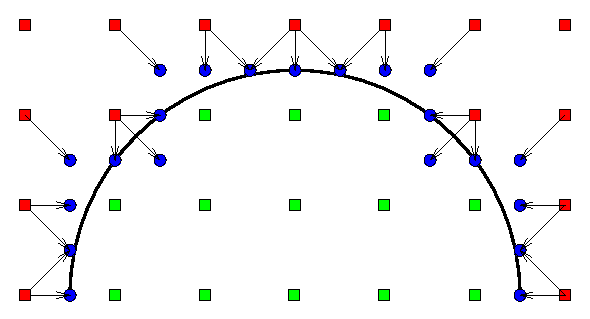
\includegraphics{xfig/colloidhalflinksnew.eps}
\end{center}
\caption{Boundary links for a colloidal particle in two dimensions
with D2Q9 (half the particle is shown). Links join fluid sites (red)
to solid sites (green) and
intersect the circular shell radius $a_0$. Boundary nodes (circles)
lie exactly half way between pairs of lattice nodes. The generalisation
to three dimensions is straightforward.}
\label{fig_coll2}
\end{figure}

A \textit{boundary node} halfway between fluid nodes which are joined
by a boundary link. The position of the boundary node is always
exactly halfway along the boundary link ($\mathbf{r} + \frac{1}{2}\mathbf{c}_b
\Delta t$) regardless of the actual position of the intersection
of the colloid surface and the boundary link.
The colloid therefore has a discrete representation which becomes a
better approximation to the sphere as the input radius becomes larger;
this approximation is known to be reasonably good for $a_0 > 5\Delta x$.



\subsubsection{Bounce-back on links}

The standard boundary condition required for the solid-fluid
interface of a moving particle is described by Ladd \cite{l94b},
and is generally refered to as bounce-back on links (BBL).
A boundary link is defined as joining a node $\mathbf{r}$
inside the particle to one outside at $\mathbf{r} + \mathbf{c}_b \Delta t$.
If the post-collision distributions are denoted by $f^\ast$, then
the distributions must be reflected at the solid surface so that
\begin{equation}
\label{eq:bbl1}
f_{b'}(\mathbf{r}; t + \Delta t) = f_b^\ast (\mathbf{r}; t)
- \frac{2w_{c_b} \rho \mathbf{u}_b.\mathbf{c}_b}{c_s^2}
\end{equation}
where the boundary link $\mathbf{c}_{b'} = -\mathbf{c}_b$. The velocity
at the boundary
\begin{equation}
\label{eq:ub}
\mathbf{u}_b = \mathbf{U} + \mathbf{\Omega}\times\mathbf{r}_b
\end{equation}
is determined by the particle linear velocity $\mathbf{U}$ and angular
velocity $\mathbf{\Omega}$. The change in momentum described by

The force exerted on a
single link is
\begin{equation}
\mathbf{F}_b(\mathbf{r} + {\scriptstyle\frac{1}{2}}\mathbf{c}_b\Delta t;
t + {\scriptstyle\frac{1}{2}}\Delta t) = \frac{\Delta x^3}{\Delta t}
\Big[ 2f_b^\ast(\mathbf{r}; t) - \frac{2w_{c_b}\rho_0 \mathbf{u}_b .
\mathbf{c}_b}{c_s^2} \Big] \mathbf{c}_b,
\label{eq:fb}
\end{equation}
with corresponding torque $\mathbf{T}_b = \mathbf{r}_b \times \mathbf{F}_b$.




The total hydrodynamic force on the particle is then found by taking
the sum of
$\mathbf{F}_b$ over all the boundary links defining the particle.
The is an associated torque on each link of $\mathbf{r}_b\times\mathbf{F}_b$,
which again is summed over all links to give the total torque on the colloid.

Note that $\rho$ in the above equations is the density of the fluid
at the appropriate fluid node for the link. As the density fluctuations
in the fluid are small compared with the mean density $\rho_0$, the
density in the correction to the bounce-back can be replaced by the
mean $\rho_0$.


\subsubsection{Dynamics}
Having computed the total force and torque on an individual colloid,
is is possible to update the the linear velocities
\begin{equation}
m_0 \mathbf{U}(t + \Delta t) = m_0 \mathbf{U}(t) + \Delta t \mathbf{F} (t),
\end{equation}
where the mass of the colloid is related to the input radius by
$m_0 = {\scriptstyle\frac{4}{3}}\pi\rho_0 a_0^3$ and the angular
velocity
\begin{equation}
I_0 \mathbf{\Omega} (t + \Delta t) = I_0 \mathbf{\Omega}(t) + \Delta t
\mathbf{T}(t),
\end{equation}
where the moment of inertia is $I_0 = {\scriptstyle\frac{2}{5}}m_o a_o^2$.
However, this explicit update is generally found to have poor stability
properties \cite{l94b, nl02}. The alternative is to use a velocity update
which is implicit \cite{heemels,nl02}.



The total force and torque on a colloid can be split into velocity-dependent
and -independent parts by combining Equations~(\ref{eq:ub})
and~(\ref{eq:fb}) to eliminate the boundary velocity $\mathbf{u}_b$.
In this way, the decomposition is
\begin{eqnarray}
\mathbf{F} = \mathbf{F}_0 - \boldsymbol{\zeta}^{FU}.\mathbf{U}
-\boldsymbol{\zeta}^{F\Omega}.\mathbf{\Omega},
\label{eq:d3}
\\
\mathbf{T} = \mathbf{T}_0 - \boldsymbol{\zeta}^{TU}.\mathbf{U}
-\boldsymbol{\zeta}^{T\Omega}.\mathbf{\Omega}.
\label{eq:d4}
\end{eqnarray}
The velocity independent parts of the force and the torque
(appropriate for a colloid at rest) are
\begin{eqnarray}
\mathbf{F}_0(t + {\scriptstyle\frac{1}{2}}\Delta t) =
\frac{2\Delta x^3}{\Delta t} \sum_b \big[ f_b^\ast(\mathbf{r}; t)
- f_{b'}^\ast(\mathbf{r} + \mathbf{c}_i \Delta t; t) \big] \mathbf{c}_b,
\\
\mathbf{T}_0(t + {\scriptstyle\frac{1}{2}}\Delta t) =
\frac{2\Delta x^3}{\Delta t} \sum_b \big[ f_b^\ast(\mathbf{r}; t)
- f_{b'}^\ast(\mathbf{r} + \mathbf{c}_i \Delta t; t) \big]
(\mathbf{r}_b\times \mathbf{c}_b)
\end{eqnarray}
The matrices $\boldsymbol{\zeta}$ are interpreted as drag
coefficients and can be written as
\begin{eqnarray}
\mathbf{\boldsymbol{\zeta}}^{FU} &=& \frac{4\rho_0 \Delta x^3}{c_s^2 \Delta t}
\sum_b w_{c_b} \mathbf{c}_b \mathbf{c}_b,
\\
\mathbf{\boldsymbol{\zeta}}^{F\Omega} &=&
\frac{4\rho_0 \Delta x^3}{c_s^2 \Delta t}
\sum_b w_{c_b} \mathbf{c}_b (\mathbf{r}_b \times \mathbf{c}_b),
\\
\mathbf{\boldsymbol{\zeta}}^{TU} &=& \frac{4\rho_0 \Delta x^3}{c_s^2 \Delta t}
\sum_b w_{c_b} (\mathbf{r}_b \times \mathbf{c}_b) \mathbf{c}_b,
\\
\mathbf{\boldsymbol{\zeta}}^{T\Omega} &=&
\frac{4\rho_0 \Delta x^3}{c_s^2 \Delta t}
\sum_b w_{c_b} (\mathbf{r}_b \times \mathbf{c}_b)
(\mathbf{r}_b \times \mathbf{c}_b).
\end{eqnarray}
As an example, the full form of the $\boldsymbol{\zeta}^{F\Omega}$ matrix is

\begin{equation}
\label{eq:k14}
\left( \begin{array}{rrr}
\sum_b c_{bx} (\mathbf{r}_b \times \mathbf{c}_b)_x &
\sum_b c_{bx} (\mathbf{r}_b \times \mathbf{c}_b)_y &
\sum_b c_{bx} (\mathbf{r}_b \times \mathbf{c}_b)_z \\

\sum_b c_{by} (\mathbf{r}_b \times \mathbf{c}_b)_x &
\sum_b c_{by} (\mathbf{r}_b \times \mathbf{c}_b)_y &
\sum_b c_{by} (\mathbf{r}_b \times \mathbf{c}_b)_z \\

\sum_b c_{bz} (\mathbf{r}_b \times \mathbf{c}_b)_x &
\sum_b c_{bz} (\mathbf{r}_b \times \mathbf{c}_b)_y &
\sum_b c_{bz} (\mathbf{r}_b \times \mathbf{c}_b)_z \\

\end{array} \right).
\end{equation}
If the particle has a symmetric distribution of boundary links (the
special case where the centre of mass is on a symmetry point of the
lattice) the $\boldsymbol{\zeta}^{FU}$ and
$\boldsymbol{\zeta}^{T\Omega}$ matrices are
diagonal, while the $\boldsymbol{\zeta}^{F\Omega}$
and $\boldsymbol{\zeta}^{TU}$ matrices are zero.

The velocity updates can now be rewritten using an
implicit update, which results in
\begin{eqnarray}
\label{eq:k15}
m_0 \mathbf{U}(t + \Delta t) = m_0 \mathbf{U}(t) + \Delta t
\big[ \mathbf{F}_0 (t + {\scriptstyle\frac{1}{2}}\Delta t)
- \boldsymbol{\zeta}^{FU} . \mathbf{U}(t + \Delta t)
- \boldsymbol{\zeta}^{F\Omega}.\mathbf{\Omega}(t + \Delta t) \big],
\\
\label{eq:k16}
I_0 \mathbf{\Omega} (t + \Delta t) = I_0 \mathbf{\Omega}(t) + \Delta t
\big[ \mathbf{T}_0(t + {\scriptstyle\frac{1}{2}} \Delta t)
- \boldsymbol{\zeta}^{TU} . \mathbf{U}(t + \Delta t)
- \boldsymbol{\zeta}^{T\Omega}. \mathbf{\Omega}(t + \Delta t) \big].
\end{eqnarray}
In general all the matrix elements are non-zero, in which case
equations~(\ref{eq:k15}) and~(\ref{eq:k16}) can be solved via a
6$\times$6 matrix inversion.

Finally, the position of the particle can be updated: an Euler
forward step is taken using the updated velocity
\begin{equation}
\mathbf{r} (t + \Delta t) = \mathbf{r} (t) + \Delta t\mathbf{U}(t + \Delta t)
\end{equation}


\subsubsection{Changes in particle shape}

One consequence is that the discrete shape of the particle fluctuates
as the colloid centre moves relative to the
lattice. This means that the size of the particle as seen by the
fluid changes despite the fact that the input radius of the colloid
is fixed.  However, these fluctuations are small for input radii
greater than about 5 lattice units \cite{l96a}. Furthermore, the
fluctuations may be greater for some input radii than others
\cite{nl02}.


In the standard approach, changes in the map of boundary links
are accomodated by the internal fluid. If the particle shape
changes so that an internal node is exposed, the internal fluid
at that site rejoins the fluid proper with the solid body momentum
(assuming the internal fluid is relaxed to solid-body rotation).
If a fluid node is covered by particle movement, then it simply
joins the internal fluid, and will relax to solid-body rotation.
Without internal fluid, changes in particle shape
in which fluid nodes are either covered or uncovered must be
accompanied by the removal or addition
of fluid with appropriate properties at the nodes in question.
It is essential that this
is done in a way which minimises the perturbation to the fluid
flow.


If a fluid node at $\mathbf{r}$ is covered by the movement of a
solid particle,
the fluid loses a mass $\rho(\mathbf{r}) \Delta x^3$, of which an excess
$\Delta M_c = (\rho(\mathbf{r}) - \rho_0)\Delta x^3$ must be replaced
explicitly so that
the overall mass density is unchanged. At the same time, the
colloid must assume the momentum lost by the fluid
$\Delta x^3 \sum_i f_i(\mathbf{r}) \mathbf{c}_i$.

Similarly, when a fluid node is exposed by particle movement,
fluid must be replaced with the appropriate distribution, density
and velocity. If the
new density is $\rho$ (to be determined by some method) then
the fluid gains an excess of mass $\Delta M_u = (\rho - \rho_0)
\Delta x^3$ which must be balanced elsewhere. If the new fluid
is assumed to have velocity $\mathbf{u}$ then the particle must
give up momentum $\Delta x^3 \rho\mathbf{u}$.

Following Nguyen and Ladd \cite{nl02}, these changes owing
to change in particle shape are implemented by added a small
correction to the bounce-back at the following time step.
The excess mass from a covered fluid site is redistributed over all the
boundary nodes by redefined the mometum transfer at bounce-back
\begin{equation}
f_{b'}(\mathbf{r}; t + \Delta t) = f_b^\ast (\mathbf{r}; t)
- \frac{2 w_{c_b} \rho_0 \mathbf{u}_b . \mathbf{c}_b}{c_s^2}
+ \frac{w_{c_b} \rho_0\Delta M_c }{A},
\label{eq:q1}
\end{equation}
where $A = \rho_0 \Delta x^3 \sum_b w_{c_b}$. The accompanying
force on the particle owing to the change in shape is then
that lost by the fluid plus the contributions from the final term
in (\ref{eq:q1}) summed over all the boundary links
\begin{equation}
\Delta \mathbf{F}_c = \frac{\Delta x^3}{\Delta t}\sum_{i} f_i \mathbf{c}_i
+ \frac{\Delta x^3}{\Delta t} \sum_b \frac{w_{c_b} \rho_0 \Delta M_c}{A}
\mathbf{c}_b.
\label{eq:q2}
\end{equation}

Note that for a closed surface,
$\sum_b w_{c_b}\mathbf{c}_b = 0$, and the second term on the right-hand
side of Eq.~(\ref{eq:q2}) is zero, i.e., the redistribution of mass
does not contribute to the net force and torque on the particle.
The corresponding change in torque is
\begin{equation}
\Delta \mathbf{T}_c = \frac{\Delta x^3}{\Delta t} \mathbf{r}_c
\times \sum_i f_i \mathbf{c}_i
+ \frac{\Delta x^3}{\Delta t}
\sum_b \frac{w_{c_b}\rho_0 \Delta M_c}{A} \mathbf{r}_b \times \mathbf{c}_b,
\label{eq:q2a}
\end{equation}
where $\mathbf{r}_c$ is the boundary vector at the position where the
fluid has been removed. Again, for a closed surface, the
redistribution of mass does not contribute to the net torque
on the particle.

Likewise, the contribution to the bounce-back from newly uncovered nodes
is
\begin{equation}
- \frac{w_{c_b} \rho_0 \Delta M_u}{A}
\label{eq:q3}
\end{equation}
leading to a change in force of
\begin{equation}
\Delta \mathbf{F}_u = -\frac{\Delta x^3 \rho(\mathbf{r})
\mathbf{u}(\mathbf{r})}{\Delta t} - \frac{\Delta x^3}{\Delta t} \sum_b
\frac{w_{c_b} \rho_0 \Delta M_u}{A} \mathbf{c}_b,
\label{eq:q4}
\end{equation}
with a corresponding change in the torque.
If more than one lattice node is either covered or uncovered by
the movement of the particle, then these contributions add in a simple
way. The overall contributions can be added to the
velocity-independent terms $\mathbf{F}_0$ and $\mathbf{T}_0$ appearing in
Equations~(\ref{eq:d3}) and~(\ref{eq:d4}).



\subsubsection{Particles near contact}

Particles near contact may not pocess a full set of boundary
links (see Figure~\ref{fig:f5}). This leads to a potential
non-conservation of mass associated with the particle motion
which must be corrected.


\begin{figure}[tb]
\begin{center}
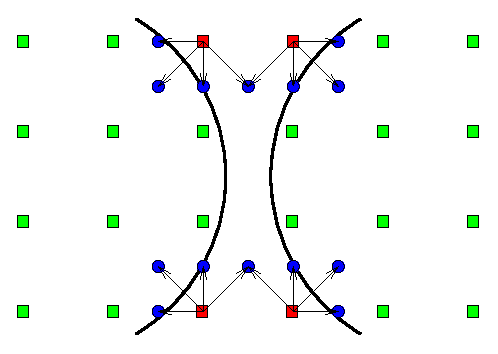
\includegraphics{xfig/colloidclose.eps}
\end{center}
\caption{Two colloids close to contact are missing links in the
region of closest approach owing to a lack of fluid nodes in the
interstice.}
\label{fig:f5}
\end{figure}
Again following Nguyen and Ladd \cite{nl02}, mass conservation is
enforced explicitly using the following procedure. There is a mass
transfer associated with the bounce-back at each link of
$(2w_{c_b}\rho_0 \mathbf{u}_b . \mathbf{c}_b / c_s^2) \Delta x^3$.
The net mass transport into the particle is the sum of this
quantity over all the links, and can be written
\begin{equation}
\Delta M_s = - \frac{2\Delta x^3 \rho_0}{c_s^2}
\Big[ \mathbf{U}.\sum_b w_{c_b} \mathbf{c}_b +
  \mathbf{\Omega} . \sum_b w_{c_b} \mathbf{r}_b \times \mathbf{c}_b \Big].
\end{equation}
For any partilce with a full set of boundary links, both
$\sum_b w_{c_b} \mathbf{c}_b$
and $\sum_b w_{c_b} \mathbf{r}_b \times \mathbf{c}_b$ are zero.
However, if the set of boundary links is imcomplete
(as in Figure~\ref{fig:f5}) $\Delta M_s$ is not zero and
a correction is required. This is again made by redistributing the
excess or deficit of mass over the other existing boundary nodes.
The additional contribution to the bounce-back here is
$-w_{c_b} \rho_0 \Delta M_s/A$, where
$A = \rho_0 \Delta x^3 \sum_b w_{c_b}$ (cf.\ Equation~\ref{eq:q1}).

This contribution
now adds to the velocity-dependent part of the force and torque and
leads to a slightly different form of the drag matrices
\begin{eqnarray}
\boldsymbol{\zeta}^{FU} &=& \frac{-2\rho_0 \Delta x^3}{c_s^2 \Delta t}
\sum_b w_{c_b} (\mathbf{c}_b - \overline{\mathbf{c}_b}) \mathbf{c}_b
\\
\boldsymbol{\zeta}^{F\Omega} &=& \frac{-2\rho_0 \Delta x^3}{c_s^2 \Delta t}
\sum_b w_{c_b} \mathbf{c}_b (\mathbf{r}_b \times \mathbf{c}_b -
\overline{\mathbf{r}_b\times\mathbf{c}_b}),
\\
\boldsymbol{\zeta}^{TU} &=& \frac{-2\rho_0 \Delta x^3}{c_s^2 \Delta t}
\sum_b w_{c_b} (\mathbf{r}_b\times\mathbf{c}_b)
(\mathbf{c}_b - \overline{\mathbf{c}_b}),
\\
\boldsymbol{\zeta}^{T\Omega} &=& \frac{-2\rho_0 \Delta x^3}{c_s^2 \Delta t}
\sum_b w_{c_b} (\mathbf{r}_b\times\mathbf{c}_b)
(\mathbf{r}_b\times\mathbf{c}_b - \overline{\mathbf{r}_b\times\mathbf{c}_b}).
\end{eqnarray}
The mean quantities
\begin{equation}
\overline{\mathbf{c}_b} = \frac{\sum_b w_{c_b} \mathbf{c}_b}{ \sum_b w_{c_b}}
\end{equation}
and
\begin{equation}
\overline{\mathbf{r}_b\times\mathbf{c}_b} =
\frac{\sum_b w_{c_b} \mathbf{r}_b\times\mathbf{c}_b}{\sum_b w_{c_b}}.
\end{equation}
A little algebra will show that both occurances of $\mathbf{c}_b$ and/or
$\mathbf{r}_b\times\mathbf{c}_b$ in the definition of the drag matrices
can be replaced by their deviation from the mean. This provides a
convenient way to compute the drag matrices (maintaining symmetry)
and computing the correct force and torque on the particle when close
to contact.



\subsubsection{Rotational motions}


For a number of applications it is useful to update not only
the psoition of a spherical particle, but its orientation. This
is important, e.g., when considering magnetic particles. The
best way to implementment the required rotations is by
considering quaternions.

A quaternion can be thought of as an extended complex number
\begin{equation}
q = w + xi + yj + zk
\end{equation}
where $i^2 = j^2 = k^2 = -1$ and $ijk = -1$. The norm, or length
of a quaternion is
\begin{equation}
N(q) = (w^2 + x^2 + y^2 + z^2)^{1/2}.
\end{equation}
Addition and subtraction of quaternions proceeds as normal, but
care is required for multiplication, which is associative but not
commutative. If the quaternion is writen as $q = (w, {\bf v})$ where
$\bf{v}$ is a normal 3-vector, then multiplication can be written
\begin{equation}
q_1 q_2 = (w_1 w_2 - {\bf v}_1 . {\bf v}_2, w_1 {\bf v}_2 + w_2 {\bf v}_1
+ {\bf v}_1 \times {\bf v}_2),
\end{equation}
where the usual scalar and vector products are used. Note that the
conjugate of a quaterion $q^\star = (w, -{\bf v})$ so that
$qq^\star = N^2(q)$.
It can be shown that a rotation of an arbitrary vector though an
angle $\theta$ around the unit axis of rotaion $\hat{\bf w}$ can
be represented by the quarternion
\begin{equation}
q = (\cos(\theta/2), \hat{\bf w} \sin(\theta/2))
\end{equation}
which ensures that $N(q) = 1$. If the arbitrary vector is (0, {\bf v}),
then the rotated vector ${\bf v}^{'}$ can be written as
\begin{equation}
(0, {\bf v}^{'}) = q (0, {\bf v}) q^\star
\end{equation}
which can be expanded as
\begin{equation}
{\bf v}^{'} = (1 - \cos\theta)({\bf v}.{\hat{\bf w}) \hat{\bf w} +
{\bf v}\cos\theta} + (\hat{\bf w} \times {\bf v})\sin\theta.  
\end{equation}


\subsection{Colloid-Colloid interactions}

\subsubsection{Lubrication corrections}

\subsubsection{Hard sphere interaction}

Particles do not overlap, i.e., there is always
a hard-sphere interaction which is a function of the separation $h$:
\begin{equation}
v^{hs}(h) = \left\{
\begin{array}{ll}
\infty & h \leq 0,\\
0   & h > 0.
\end{array} \right.
\end{equation}
The hard-sphere interaction does not give rise to a force.


\subsubsection{Soft-sphere interaction}

A simple soft-sphere interaction is available, the basic form
of which is:
\begin{equation}
v^{ss}(r) = \epsilon (\sigma / r)^{\nu},
\end{equation}
where $\epsilon$ sets the energy scale, and $\sigma$ sets the
characteristic width. The steepness of the potential is set by
the exponent $\nu (> 0)$.

To prevent the need for calculation of long-range interactions,
the soft-sphere potential is truncated in a ``cut-and-shift''
approach. This is done in such a way as to smoothly match
both the potential and the force at the cut-off distance
$r_c$. For $r < r_c$ the potential is then
\begin{equation}
v^{ss}(r) - v^{ss}(r_c) - (r - r_c) \left.\frac{d v^{ss}}{dr}\right|_{r=r_c}.
\label{eq_ss_shift}
\end{equation}
Clearly, this potential is not exactly what we first thought of as
soft-sphere. Matching the potential smoothly ensures conservation
of energy, while matching the force smoothly prevents potential
instabilities in the molecular dynamics update.

The soft-sphere potential can be useful as a mechanism to
keep the particles from touching (which risks hard-sphere interactions),
in which case is is possible to compute the interaction as a function
of the separation $h$, instead of $r$. The force between
two particles is computed via the derivative of equation~\ref{eq_ss_shift}
with respect to $r$:
\begin{equation}
\mathbf{F}_{ij}(r) = -\left\{\frac{d v^{ss}(r)}{dr} -
\left. \frac{d v^{ss}(r)}{dr}\right|_{r=r_c} \right\} \mathbf{\hat{r}}_{ij}
\end{equation}
where $\mathbf{\hat{r}}_{ij}$ is the unit vector joining the centre of
particle $i$ to the centre of $j$.



\subsubsection{Leonard-Jones interaction}



\section{Lattice Boltzmann for a Binary Fluid}

\subsection{The Cahn-Hilliard Equation}

\subsection{The Choice of Free Energy}

\subsection{A Second Distribution Function}

\subsection{The Collision}

\subsection{Bounce-Back on Links}




\section{Surfactants}

This section describes the approach taken to study surfactants. Here,
we always adopt the hydrid method, i.e., LB for the hydrodynmic
equations and finite difference for the associated Cahn-Hilliard
equations. Coupling between the two sectors is via the velocity
field and the external force on the fluid computed via the
divergence of the `chemical stress'.

In this model the surfactant appears as a concentration field
$\psi(\mathbf{r};t)$, alongside the compositional order parameter
$\phi(\mathbf{r};t)$ as appears in the binary fluid. There are
two corresponding Cahn-Hilliard equations: first,

\begin{equation}
\partial_t \phi + \partial_\alpha \phi u_\alpha = 
\partial_\alpha M_\phi \partial_\alpha \mu_\phi,
\end{equation}
and second
\begin{equation}
\partial_t \psi + \partial_\alpha \psi u_\alpha = 
\partial_\alpha M_\psi \partial_\alpha \mu_\psi.
\end{equation}

\subsection{Free Energy}

A number of different free energies have been used to study
surfactants [cite Yeomans]. Here, the free energy is based on
that used by van der Graff and van der Sman and others [cite].
There are a number of different contributions to the free
energy density:
\begin{equation}
f = f_\phi + f_\psi +f_1 + f_{ex}.
\end{equation}
The first is exactly that used for the binary fluid, i.e.,
\begin{equation}
f_\phi (\phi, \partial_\alpha\phi) =
{\textstyle \frac{1}{2}} A \phi^2 + {\textstyle \frac{1}{4}} B \phi^4
+ {\textstyle \frac{1}{2}} \kappa (\partial_\alpha \phi)^2.
\end{equation}
The surface tension and the interfacial width are determined from the
choice of parameters $A,B,\kappa$ as before.
The second term in the free energy density
represents the entropic
energy of mixing of the surfactant with the bulk phases
\begin{equation}
f_\psi (\psi) = kT \left[ \psi \ln\psi + (1 - \psi)\ln(1-\psi) \right]
\end{equation}
where the parameter $kT$ sets the energy scale for the whole system.
The surfactant order parameter, $\psi$, is unity for a saturated
interface and zero for a plain interface.

The surfactant lowers the energy of the interface where it is adsorbed
there, represented by the term
\begin{equation}
f_1(\psi, \partial_\alpha \phi) 
= -{\textstyle \frac{1}{2}} \epsilon \psi (\partial_\alpha \phi)^2
  -{\textstyle \frac{1}{2}} \beta  \psi^2 (\partial_\alpha \phi)^2
\end{equation}
where $\epsilon$ and $\beta$ are parameters. Note that only the
first term appears in \cite{vandergraaf}, while the second term is
based on that appearing in, e.g., \cite{diamant}. If $\beta = 0$,
the surfactant profile at the interface is symmetric (so-called
Langmuir adsoption) whereas the term in $\beta$ induces an
asymmetry (Frumpkin adsorption).
Finally,  $f_{ex}$ is [van der Sman claims]
an enthalpic contribution introduced 
to stabilise the interface \cite{theissengompper}
\begin{equation}
f_{ex} (\psi, \partial_\alpha \phi) = {\textstyle\frac{1}{2}} W \psi \phi^2,
\end{equation}
with $W$ a parameter.

\subsection{Chemical potentials}

The respective chemical potentials are obtained from the functional
derivatives of the free energy $\mu_\phi = \delta F / \delta \phi$ and
$\mu_\psi = \delta F / \delta \psi$. We obtain:
\begin{equation}
\mu_\phi =
A\phi + B\phi^3 -\kappa \partial_\alpha^2 \phi
+ W\psi\phi + \epsilon\psi\partial_\alpha^2 \phi
+ \epsilon \partial_\alpha \phi \partial_\alpha \psi
+ 2\beta \psi\partial_\alpha\phi \partial_\alpha \psi
+ \beta \psi^2 \partial_\alpha^2 \phi,
\end{equation}
and
\begin{equation}
\mu_\psi = kT \left[ \ln\psi - \ln(1-\psi) \right]
+ {\textstyle \frac{1}{2}}W\phi^2
- {\textstyle \frac{1}{2}}\epsilon (\partial_\alpha \phi)^2
- \beta\psi (\partial_\alpha \phi)^2.
\end{equation}
As before, the pressure tensor is $P_{\alpha\beta} = p_0\delta_{\alpha\beta}
+ \tilde{P}_{\alpha\beta}$ with the isotropic part being determined as (e.g.,
\cite{theissengompper})
\begin{equation}
p_0 = \phi \mu_\phi + \psi \mu_\psi - f(\phi, \psi, \partial_\alpha \phi).
\end{equation}
There is no closed form for the tensor part, which must be chosen to
comply with the constraint that in mechanical equilibrium
\begin{equation}
\partial_\alpha P_{\alpha\beta} = (\phi\partial_\alpha\mu_\phi +
\psi\partial_\alpha\mu_\psi)\delta_{\alpha\beta}.
\end{equation}
In this way we obtain for the isotropic contribution
\begin{eqnarray}
p_0 = {\textstyle \frac{1}{2}}A\phi^2 + {\textstyle \frac{3}{4}}B\phi^4 
- {\textstyle\frac{1}{2}}\kappa (\partial_\alpha\phi)^2 
- \kappa \phi \partial_\alpha^2 \phi
- kT \ln(1-\psi) + W\psi\phi^2
\nonumber\\
+ \epsilon \phi \partial_\alpha \phi \partial_\alpha \psi
+ \epsilon\phi\psi \partial_\alpha^2 \phi
+ 2 \beta\phi\psi \partial_\alpha \phi \partial_\alpha\psi
+ \beta \phi \psi^2 \partial_\alpha^2 \phi
- {\textstyle\frac{1}{2}} \beta \psi^2 (\partial_\alpha \phi)^2
\end{eqnarray}
and for the tensor part we can have
\begin{equation}
\tilde{P}_{\alpha\beta} =
(\kappa - \epsilon \psi - \beta\psi^2) 
\partial_\alpha \phi \partial_\beta \phi.
\end{equation}




\section{Code Design}

\subsection{Some Comments}

In designing a code in C the main object of which is to do high
performance computing, there are some inevitable tensions with
software engineering best-practice. In particular, complete
encapsulation of data in the spirit of using abstract data types
tends to cause problems of performance.

For example, encapsulation of the lattice Boltzmann distribution
$f_i$, together with appropriate ``get'' and ``set'' functions for
access when approapriate, is possible. There could then be a
complete separation of interface and implementation of the
distribution (other than that each individual $f_i$ is represented
by a \texttt{double}). However, experience suggests that
this imposes severe impediment to optimisation and hence
unacceptable performance degradation.

Schemes do exist by which one can approximate the object
oriented programming style in C, and so achieve a separation
of interface and implementation. However, this tends to put
a heavy burden on the use of \texttt{void} pointers, itself
a recipe for possible disaster. A truly object-oriented
language such as Java would be preferable.

So, for the time being, some relaxation of encapsulation is required.
Exposing a pointer to the distributions which allows them to be accessed
directly where required. This can be done merely by declaring the
necessary variables \texttt{extern}. In practice, such deviations
from encapsulation can be minimised in the lattice sector of the
code. In particlar, \texttt{extern} declarations should not be
required in \texttt{main()}, i.e., it should be able to write a
new application without worrying about details of implementation.

\subsubsection{Objects}

Somewhat more difficult is the part of the code involving
colloids, which would really favour a truly object-oriented
approach.

\subsubsection{Serial and parallel}

The design decission has been taken to support execution of the
code in both serial and parallel. The default compilation
assumes that a serial executable is required, while  MPI code
is introduced via C-preprocessor directives (\texttt{-D\_MPI\_}).


There is no shared memory inplementation at this time.


\subsection{Structural Components: \texttt{MPI\_COMM\_WORLD}}


\subsection{Coordinate System: \texttt{MPI\_CARTESIAN\_COMMUNICATOR}}


\begin{figure}
\begin{center}
%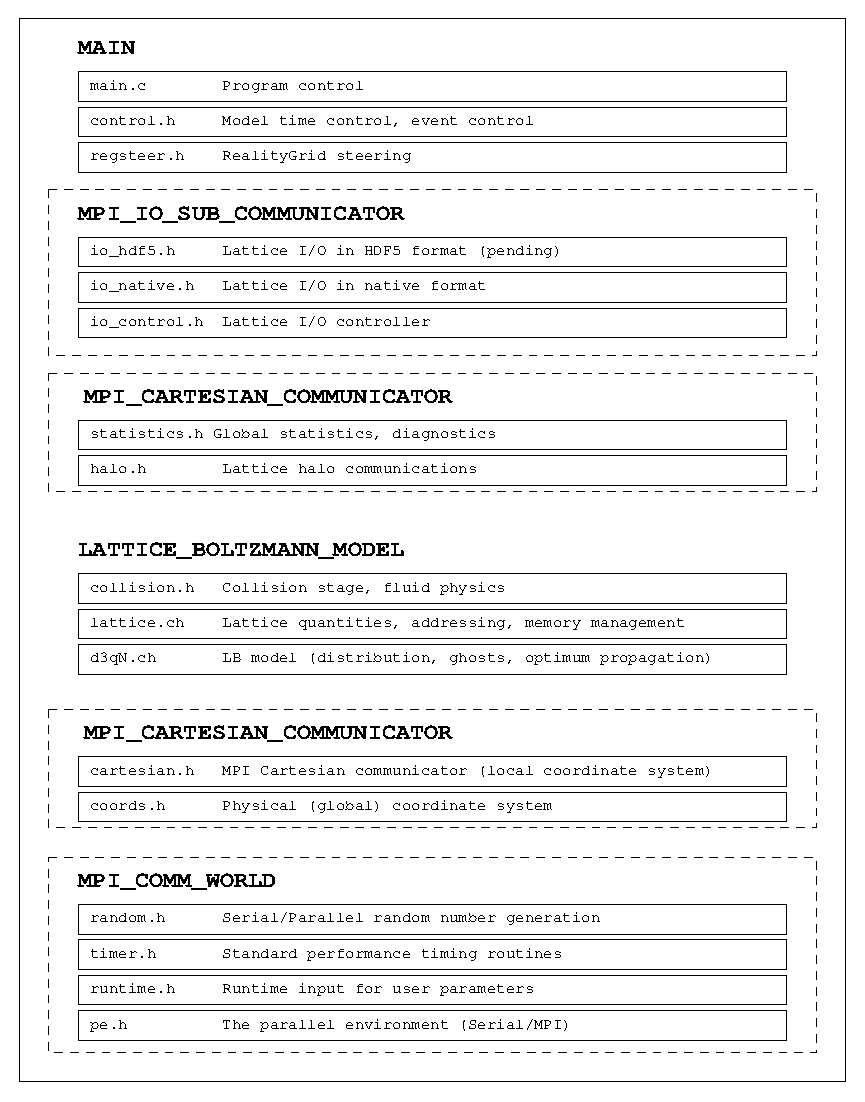
\includegraphics{xfig/sketch.eps}
\end{center}
\caption{A scheme by which different parts of the code might be
encapsulated and in such a way to allow reliable development and
testing. As this is C, will do not adopt a truly ``object'' langauge.
Broadly, different modular parts should only depend on stuff above
in the diagram. So, at the top, there is the parallel environment
where communication occurs within MPI\_COMM\_WORLD. Built on top
of this is the Cartesian Communicator responsible for halo swaps
and so forth. The LE code may have a separate Communicator again. 
(There's an argument to say the diagram should be the other way up!)}
\end{figure}



\section{Code Implementation}

\subsection{Stuff}

\subsection{Coordinate System}

\subsubsection{The global coordinate system}

The user specifies the system size in lattice units at run time,
which sets the extent of memory which must be allocated for the
Cartesian lattice. The extent of the physical coordinate system
then reflects the lattice size directly (see Figure \ref{fig_c1}). 
Each lattice site, or node,  has coordinates corresponding to its
integer position in the system and can be thought of as being
at the centre of a control volume one lattice unit on a side.
This means that the nominal edges of the
system are offset from the lattice sites themselves by half a
lattice unit in each direction.


\begin{figure}[h]
\begin{center}
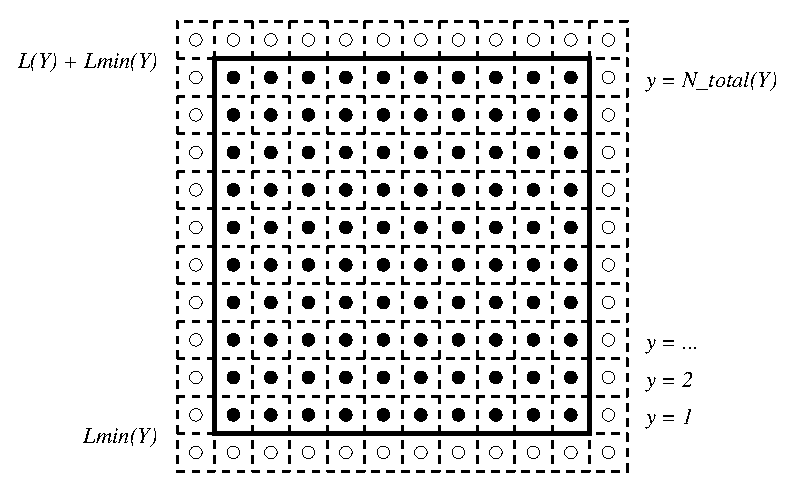
\includegraphics{xfig/fig_c1.eps}
\end{center}
\caption{The global Cartesian coordinate system reflects the choice
of lattice size; lattices sites are located at
$x=1, \ldots, x = N_{total}$ and so on in each coordinate direction
(the Figure only shows the labels in the $y-$direction for simplicity).
In the Figure, the lattice sites in the domain proper are the full
circles; halo sites, which are used to effect periodic boundary
conditions, are included as open cirles}
\label{fig_c1}
\end{figure}

For particles, the centres of which can move continuously across the
lattice, the extents of the global coordinate system are then
$L_{min} < x < L + L_{min}$ and so on.

\subsubsection{Addressing the lattice: the local coordinate system}


\subsection{Solid walls}

General solid objects which are fixed for the duration of
the simulation, such as porous media, can be defined
by assigning solid/fluid status to each lattice node. 
The links required between solid and fluid nodes can
then be identified for the given model.

\textit{Comment.} In general, a solid object will not
affect the periodic nature of the simulation. A general
solid object cannot move, i.e., the boundary velocity
must be zero.

\textit{Special case.} In the case where the solid object
represents a flat boundary wall at the edge of the system
in one or more directions, the periodicity is broken in
the corresponding directions.


\vfill
\pagebreak

\section{Code Interface}

\subsection{The Parallel Environment}

\texttt{\#include ``pe.h''}

As the code is to be available in both serial and parallel versions,
it is desirable to abstract the basic environment to some extent.
The parallel environment is intended to support MPI communication
within \texttt{MPI\_COMM\_WORLD}, or fall back to a minimally
consistent picture in serial (i.e., rank zero is the single process).

\texttt{void pe\_init(int argc, char ** argv)}\\
Responsible for initialisation of MPI, and hence must be first
execuatable statement. The arguments are those to \texttt{main}
which will be passed through to \texttt{MPI\_Init()}.

\texttt{int pe\_rank(void)}\\
Returns the process rank in \texttt{MPI\_COMM\_WORLD}, or 0 in
serial.

\texttt{int pe\_size(void)}\\
Returns the number of processes in \texttt{MPI\_COMM\_WORLD}, or
1 in serial.

\texttt{void pe\_finalise(void)}\\
Responsible for \texttt{MPI\_Finalize()}, and must be the last
executable statement.

\texttt{void info(const char * fmt, ...)}\\
Behaves like \texttt{printf}, but only produces output on the
root process.

\texttt{void verbose(const char * fmt, ...)}\\
Behaves as \texttt{printf} and reports the rank of the
calling process in \texttt{MPI\_COMM\_WORLD}.

\texttt{void fatal(const char * fmt, ...)}\\
Prints an error message and identifies
the rank of the calling process before terminating the program.


\subsection{Run Time Input}

\texttt{\#include ``runtime.h''}

The ability to set a wide range of parameters at run time is
very convenient, and is supported via an input file in which the
user specifies parameters as key value pairs. The code maintains
a list of key value pairs from which the user can retrieve the
appropriate values for given keys.


\texttt{void RUN\_read\_input\_file(const char * input\_file\_name)}\\
This reads the named input file and sets up the list of keys.

\texttt{int RUN\_get\_double\_parameter(const char *key, double * value)}\\
Set the \texttt{value} associated with \texttt{key}, if present. The number
of key matches found is returned (i.e., 0 or 1).

\texttt{int RUN\_get\_int\_parameter(const char * key, int * value)}\\
Set the \texttt{value} associated with \texttt{key}, if present. The
number of key matches is returned.

\texttt{int  RUN\_get\_string\_parameter(const char * key, char * value)}\\
Set \texttt{value} to the string assocaited with \texttt{key}, if
present. Returns the number of key matches found.

\texttt{int  RUN\_get\_int\_parameter\_vector(const char * key, int v[])}\\
If \texttt{key} is present, set the associated 3-vector of integers.
Returns the number of key matches found. 

\texttt{int  RUN\_get\_double\_parameter\_vector(const char * key,
double v[])}\\
If \texttt{key} is present, set the associated 3-vector of doubles.
Returns the number of key matches found.

\textit{Comment:} We probably need a function to report unused keys, so
the user can be alerted if a key has unexpectedly been ignored.


\subsection{Random Number Generators}

\texttt{\#include ``ran.h''}

Note that the random number generation in parallel is
decomposition dependent.

\texttt{void rand\_init(void)}\\
Responsible for initialising RNG state.

\texttt{double rand\_serial\_uniform(void)}\\
Return a single variate uniformly distributed on $[0,1]$ from
the serial generator.

\texttt{double rand\_serial\_gaussian(void)}\\
Return a single variate with Gaussian distribution about zero
and having unit variance from the serial generator.

\textit{double rand\_parallel\_uniform(void)}\\
Return a single variate uniformly distributed on $[0,1]$
from the serial generator.

\texttt{double rand\_parallel\_gaussian(void)}\\
Return a single variate with Gaussian distribution about zero
and having unit variance from the parallel generator.

\textit{Comment:} The serial generator will produce the
same sequence on any MPI process, while the parallel generator
will produce different sequences. The latter is intended for
generating, specifically, fluctuations, where the need for
decomposition-independance is questionable.



\subsection{Timers}

\texttt{\#include ``timer.h''}

Performance figures require timing for different sections
of the code. The code provides a set of routines to time
standard and user-defined sections of code. Timers are
started and stopped by call to the appropriate routines.

\texttt{TIMER\_init()}\\
This initialises all the timers to zero (e.g., at the start of
the program).

\texttt{TIMER\_start(const int t\_id)}\\
Start the given timer.

\texttt{TIMER\_stop(const int t\_id)}\\
Stop the given timer.

\texttt{TIMER\_statistics(void)}\\
Prints the current state of all the active timers to standard
output on the root process in a digestible form. In serial,
the minimum, maximum, and mean time for each timer is reported
in seconds (based on the number of start/stop cycles). In
parallel, the same figures are computed on each process and the
result of the corresponding \texttt{MPI\_Reduce()} operation is
printed on the root process.

The code provides a number of timers which would time standard
parts of the code, e.g., \texttt{t\_id = TIMER\_TOTAL} for the
total execution time, and a number of spare timers for users to
use at will.


\textit{Comment:}
No intra-run variance (i.e., between time steps) is provided, as the
calculation required is considerably more complex to generalise, and
requires memory proportional to the number of time steps used.


\textit{Comment:}
Two macros, \texttt{TIMER\_START()} and \texttt{TIMER\_STOP()} are
provided to insert calls to the above functions for optional timing
of performance-sensitive regions
of the code in conjunction with the preprocessor flag
\texttt{-D\_TIMING\_MACRO\_ON\_}.


\subsection{Model Time Control}

This provides time step control, event frequency (?)

\texttt{void init\_control(void)}\\
Initialise time controls.

\texttt{int get\_step(void)}\\
Return the current model time step.

\texttt{int next\_step(void)}\\
Increments the current time step. Returns number of steps left
to run (i.e., 0 when finished).



\subsection{Coordinate System}

\texttt{\#include ``coords.h''}

A three-dimensional Cartesian coordinate system is used throughout,
with the exact system size usually chosen by the user at run time.
The symbolic constants \texttt{X}, \texttt{Y}, and \texttt{Z} are
used to identify the coordinate directions.

This also provides access to the MPI Cartesian Communicator which
is responsible for most communication in the model.

\texttt{int N\_total(const int dim)}\\
Returns the total number of lattice sites in the given Cartesian direction.

\texttt{double L(const int dim)}\\
Returns the length of the system in the given Cartesian direction
(which is the same as the number of lattice sites).

\texttt{double Lmin(const int dim)}\\
Returns coordinate position of left-hand edge of system in given
Cartesian direction.

\texttt{int is\_periodic(const int dim)}\\
Returns 1 if given Cartesian direction is periodic, else 0.

\texttt{void cart\_init(void)}\\
Responsible for setting up the Cartesian decomposition.

\texttt{int cart\_rank(void)}\\
Returns rank in the Cartesian communicator.

\texttt{MPI\_Comm cart\_comm(void)}\\
Returns the MPI Communicator handle for the Cartesian communicator.

\texttt{int cart\_size(const int dim)}\\
Returns the size of the Cartesian communicator grid in the given
coordinate direcxtion.

\texttt{int cart\_coord(const int dim)}\\
Returns the coordinate of the current process in the Cartesian
Communicator.

\texttt{int cart\_neigh(const int dir, const int dim)}\\
Returns the rank of the neighbouring process in the
Cartesian communicator.


\subsection{Colloids}

\texttt{\#include ``colloids.h''}

These functions provide the basic interface for use
of colloidal particles in the code.

\subsubsection{Colloid structure}

The basic colloid struct is defined ...
 

\subsubsection{Colloid interface}

\texttt{void colloids\_init(void)}\\
Call once for initialisation. This initialises the cell list,
so the coordinate system must be initialised via a call to
\texttt{coords\_init()} first.

\texttt{void colloids\_finish(void)}\\
Call once for finalisation. Frees all colloid-related memory.

\texttt{Colloid * allocate\_colloid(void)}\\
Returns a pointer to a newly allocated \texttt{Colloid} object
or fails gracefully.

\texttt{void free\_colloid(Colloid * p\_colloid)}\\
Deallocates all memory associated with \texttt{p\_colloid} or
fails gracefully.

\texttt{struct c\_link allocate\_boundary\_link(void)}\\
Returns a pointer to a newly allocated colloid boundary
link or fails gracefully.

\texttt{void free\_boundary\_link(struct c\_link *)}\\
Deallocates memory associated with a link or fails gracefully.

\texttt{void colloids\_memory\_report(void)}\\
The module keeps track of how much memory has been allocated in
total for colloids and boundary links. This reports the current
usage.

\texttt{get\_Ncell\_total()}\\

\texttt{get\_Ncell\_local()}\\

\texttt{Colloid * cell\_get\_colloid(int i, int j, int k)}\\
This returns a pointer to the Colloid at the head of the list at
cell list location (i, j, k) or \texttt{NULL} if there is none.

\texttt{void cell\_insert(Colloid * p\_colloid)}\\
This inserts a colloid at the head of the appropriate list
depending upon its position. This is the only way a colloid
can be added to the list.

\texttt{update\_cells(void)}\\
Performs the update of the cell list in response to updated
particle positions.

\texttt{IVector cell\_coords(FVector r)}\\




\subsection{Speculation}

\subsection{The Free Energy}

It is imagined that a single file will encapsulate all the details
of a given free energy. The interface for different choices of
free energy should be the same.


\texttt{FE\_init()}

Responsible for querying the runtime input key value pair list to
find appropriate user parameters for the free energy, or
falling back to default values.


\texttt{double FE\_get\_sigma()}

Return the surface tension. There should be a similar routine
for the interfacial thickness.

\texttt{double FE\_get\_mu(const type location)}

Return the chemical potential at the single lattice
node \texttt{location}.

\textit{Comment:} The computation of quantities such as the chemical
potential will a) affect performance and b) require halo values of
the order parameter (depending on the highest derivative
in the order parameter present). Performance here should be the
first consideration, so this needs to be handled with care.


\texttt{double pchem[ND][ND] FE\_get\_pchem(const type location)}

Return the chemical stress ${\cal P}_{\alpha\beta}$ at the
given location.

\textit{Comment:} This is an $nd \times nd$ matrix, where $nd$ is
the number of dimensions. If we are to provide explicit support for
D2Q9, \texttt{ND} will be 2, otherwise 3.





\section{Implementation Notes}

\subsection{Serial Version}

\subsection{Efficiently Scaling Parallel Computing}

We should be thinking about the 100,000 processor regime, and
correspondingly large system sizes. To avoid embarrassment in this regime,
some issues which don't usually arise are relevant, for example:

\begin{enumerate}
\item
Large integer quantities such as
\begin{verbatim}
   N_total.x*N_total.y*N_total.z
\end{verbatim}
are likely to cause integer overflow (if default integers are 4 byte).
\item
Local data structures whose size is proportional
to the number of processors are contraindicated, e.g.,
anything like
\begin{verbatim}
p = (foo *) malloc(nprocs*sizeof(foo));
\end{verbatim}
is to be avoided. At the moment, we are in good shape on this
(apart from some functions in \texttt{misc.c}).
\item
I/O is likely become a very important issue, so may need to think
more about this.
\item
We should probably introduce a standard set of benchmarks which can
be scaled up in some systematic way, so that we can keep track of
performance over time.

\end{enumerate}


\section{Model Details}

\subsection{D3Q15}

These are the eigenvalues and eigenvectors of teh collision
matrix used for D3Q15


\begin{table}
\begin{tabular}{|l|r|r|rrrrrr|rrrrrrrr|r|l|}
\hline\hline
$M^a$ & & \multicolumn{15}{c|}{$m_i^a$} & $N^a$  &\\
\hline
$\rho$ & - &
 1 &  1 &  1 &  1 &  1 &  1 &  1 &  1 &  1 &  1 &  1 &  1 &  1 &  1 &  1 &
1 &$\mathbf{1}$ \\
\hline
$\rho c_{ix}$ & - &
 0 &  1 & -1 &  0 &  0 &  0 &  0 &  1 & -1 &  1 & -1 &  1 & -1 &  1 & -1 &
3  & $c_{ix}$ \\
\hline
$\rho c_{iy}$ & - &
 0 &  0 &  0 &  1 & -1 &  0 &  0 &  1 &  1 & -1 & -1 &  1 &  1 & -1 & -1 &
3  &$c_{iy}$ \\
\hline
$\rho c_{iz}$ & - &
 0 &  0 &  0 &  0 &  0 &  1 & -1 &  1 &  1 &  1 &  1 & -1 & -1 & -1 & -1 &
3  & $c_{iz}$ \\
\hline
$Q_{xx}$ & 1/3 &
-1 &  2 &  2 & -1 & -1 & -1 & -1 &  2 &  2 &  2 &  2 &  2 &  2 &  2 &  2 &
9/2  & $c_{ix} c_{ix} - c_s^2$ \\
\hline
$Q_{yy}$ & 1/3 &
-1 & -1 & -1 &  2 &  2 & -1 & -1 &  2 &  2 &  2 &  2 &  2 &  2 &  2 &  2 &
 9/2 & $c_{iy} c_{iy} - c_s^2$ \\
\hline
$Q_{zz}$ & 1/3 &
-1 & -1 & -1 & -1 & -1 &  2 &  2 &  2 &  2 &  2 &  2 &  2 &  2 &  2 &  2 &
 9/2 & $c_{iz} c_{iz} - c_s^2$ \\
\hline
$Q_{xy}$ & - &
 0 &  0 &  0 &  0 &  0 &  0 &  0 &  1 & -1 & -1 &  1 &  1 & -1 & -1 &  1 &
9  & $c_{ix} c_{iy}$ \\
\hline
$Q_{yz}$ & - &
 0 &  0 &  0 &  0 &  0 &  0 &  0 &  1 &  1 & -1 & -1 & -1 & -1 &  1 &  1 &
9  & $c_{iy} c_{iz}$ \\
\hline
$Q_{zx}$ & - &
 0 &  0 &  0 &  0 &  0 &  0 &  0 &  1 & -1 &  1 & -1 & -1 &  1 & -1 &  1 &
9  & $c_{iz} c_{ix}$ \\
\hline\hline
$\chi^1$ & - &
-2 &  1 &  1 &  1 &  1 &  1 &  1 & -2 & -2 & -2 & -2 & -2 & -2 & -2 & -2 &
1/2 & $\chi^1$ \\
\hline
$J_{ix}$ & - &
 0 &  1 & -1 &  0 &  0 &  0 &  0 & -2 &  2 & -2 &  2 & -2 &  2 & -2 &  2 &
3/2 & $\chi^1 \rho c_{ix}$\\
\hline
$J_{iy}$ & - &
 0 &   0 &  0 &  1 & -1 &  0 &  0 & -2 & -2 &  2 &  2 & -2 & -2 &  2 &  2 &
3/2 & $\chi^1 \rho c_{iy}$\\
\hline
$J_{iz}$ & - &
 0 &   0 &  0 &  0 &  0 &  1 & -1 & -2 & -2 & -2 & -2 &  2 &  2 &  2 &  2 &
3/2 & $\chi^1 \rho c_{iz}$\\
\hline
$\chi^3$ & - &
 0 &   0 &  0 &  0 &  0 &  0 &  0 &  1 & -1 & -1 &  1 & -1 &  1 &  1 & -1 &
9 & $c_{ix} c_{iy} c_{iz}$ \\
\hline\hline
$w_i$ & 1/72 &
$16$ & 8 & 8 & 8 & 8 & 8 & 8 & 1 & 1 & 1 & 1 & 1 & 1 & 1 & 1 &
 & $w_i$\\
\hline\hline
\end{tabular}
\end{table}


\subsection{D3Q19}

\begin{table}
\begin{tabular}{|l||r|rrrrrr|rrrr|rrrr|rrrr|r||}
\hline\hline
$M^a$ & \multicolumn{19}{c||}{$m_i^a$} & $N^a$\\
\hline
$\rho $ & 1 &  1 &  1 &  1 &  1 &  1 &  1 & 
         1 &  1 &  1 &   1 &  1 &  1 &  1 & 1 & 1 & 1 & 1 & 1
& 1\\
\hline
$\rho c_{ix}$ & 0 &  1 &  -1 &  0 &  0 &  0 &  0 & 
         1 &  1 &  -1 &   -1 &  1 &  1 &  -1 & -1 & 0 & 0 & 0 & 0
& 3 \\
\hline
$\rho c_{iy}$ & 0 &  0 &  0 &  1 &  -1 &  0 &  0 & 
         1 &  -1 &  1 &   -1 &  0 &  0 &  0 & 0 & 1 & 1 & -1 & -1
& 3\\
\hline
$\rho c_{iz}$ & 0 &  0 &  0 &  0 &  0 &  1 &  -1 & 
         0 &  0 &  0 &   0 &  1 &  -1 &  1 & -1 & 1 & -1 & 1 & -1
& 3\\
\hline
$Q_{ixx}$ & -1 &  2 &  2 &  -1&  -1 &  -1 &  -1 & 
         2 &  2 &  2 &   2 &  2 &  2 &  2 & 2 & -1 & -1 & -1 & -1
& 9/2\\
\hline
$Q_{iyy}$ & -1 &  -1 &  -1 &  2&  2 &  -1 &  -1 & 
         2 &  2 &  2 &   2 &  -1 &  -1 &  -1 & -1 & 2 & 2 & 2 & 2
& 9/2\\
\hline
$Q_{izz}$ & -1 &  -1 &  -1 &  -1&  -1 &  2 &  2 & 
         -1 &  -1 &  -1 &   -1 &  2 &  2 & 2 & 2 & 2 & 2 & 2 & 2
& 9/2\\
\hline
$Q_{ixy}$ & 0 &  0 &  0 &  0&  0 &  0 &  0 & 
          1 &  -1 &  -1 &    1 &  0 &  0 & 0 & 0 & 0 & 0 & 0 & 0
& 9\\
\hline
$Q_{ixz}$ & 0 &  0 &  0 &  0&  0 &  0 &  0 & 
          0 &   0 &   0 &   0 &  1 & -1 & -1 & 1 & 0 & 0 & 0 & 0
& 9\\
\hline
$Q_{iyz}$ & 0 &  0 &  0 &  0&  0 &  0 &  0 & 
          0 &   0 &   0 &   0 &  0 & 0 & 0 & 0 & 1 & -1 & -1 & 1
& 9\\
\hline\hline
$\chi^1$ & 0 &  1 &  1 &  1 &  1 &  -2 &  -2 & 
         -2 &  -2 &  -2 &  -2 &  1 &  1 & 1 & 1 & 1 & 1 & 1 & 1
& 3/4\\
\hline
$\chi^1 \rho c_{ix}$ & 0 &  1 &  -1 &  0&  0 &  0 &  0 & 
         -2 &  -2 &  2 &  2 &  1 &  1 & -1 & -1 & 0 & 0 & 0 & 0
& 3/2\\
\hline
$\chi^1 \rho c_{iy}$ & 0 &  0 &  0 &  1&  -1 &  0 &  0 & 
         -2 &  2 &  -2 &  2 &  0 &  0 & 0 & 0 & 1 & 1 & -1 & -1
& 3/2\\
\hline
$\chi^1 \rho c_{iz}$ & 0 &  0 &  0 &  0&  0 &  -2 &  2 & 
         0 &  0 &  0 &  0 &  1 &  -1 & 1 & -1 & 1 & -1 & 1 & -1
& 3/2\\
\hline
$\chi^2$ & 0 &  1 &  1 &  -1&  -1 &  0 &  0 & 
         0 &  0 &  0 &  0 &  -1 &  -1 & -1 & -1 & 1 & 1 & 1 & 1
& 9/4\\
\hline
$\chi^2 \rho c_{ix}$ & 0 &  1 &  -1 &  0&  0 &  0 &  0 & 
         0 &  0 &  0 &  0 &  -1 &  -1 & 1 & 1 & 0 & 0 & 0 & 0
& 9/2\\
\hline
$\chi^2 \rho c_{iy}$ & 0 &  0 &  0 & -1&   1 &  0 &  0 & 
         0 &  0 &  0 &  0 &   0 &  0 & 0 & 0 & 1 &  1 & -1 & -1
& 9/2\\
\hline
$\chi^2 \rho c_{iz}$ & 0 &  0 &  0 &  0&  0 &  0 &  0 & 
         0 &  0 &  0 &  0 &  -1 &  1 & -1 & 1 & 1 & -1 & 1 & -1
& 9/2\\
\hline
$\chi^3$ & 1 &  -2 &  -2 &  -2&  -2 &  -2 &  -2 & 
         1 &  1 &  1 &  1 &  1 &  1 & 1 & 1 & 1 & 1 & 1 & 1
& 1/2\\
\hline\hline
$w_i$ & 12 & 2 & 2 & 2 & 2 & 2 & 2 & 
1 & 1 & 1 & 1 & 1 & 1 & 1 & 1 & 1 & 1 & 1 & 1
& \\
\hline\hline
\end{tabular}
\end{table}



\pagebreak


\begin{thebibliography}{99}

\bibitem{adhikari2005}
Adhikari, R., K. Stratford. M.E. Cates, and A.J. Wagner,
Fluctuating Lattice Boltzmann,
\textit{Europhys. Lett.}, \textbf{71}, 473 2005.

\bibitem{ald98}
Aidun, C.K., Y. Lu, and E.-J. Ding,
Direct analysis of particulate suspensions with inertia using the
discrete Boltzmann equation,
\textit{J. Fluid Mech.}, \textbf{373}, 287, 1998.

\bibitem{chunladd}
B. Chun and A.J.C. Ladd,
Interpolated boundary condition for lattice Boltzmann simulations in
narrow gaps,
\textit{Phys. Rev. E}, \textbf{75}, 066705, 2007.

\bibitem{cj98}
Cichocki, B., and R.B. Jones,
Image representation of a spherical particle near a hard wall,
\textit{Physica A}, \textbf{258}, 273, 1998.

\bibitem{chang}
C.-H. Chang and E.I. Franses,
Adsorption dynamics of surfactants at the air/water interface:
a critical review of mathematical models, data, and mechanisms,
\textit{Colloids and Surfaces A}, \textbf{100} 1, 1995.

\bibitem{cpc}
Desplat, J.-C., I. Pagonabarraga, and P. Bladon,
LUDWIG: A parallel lattice-Boltzmann code for complex fluids.
\textit{Comput. Phys. Comms.}, \textbf{134}, 273, 2001.

\bibitem{diamant}
H. Diamant and D. Andelman,
Kinetics of surfactant adsorption at fluid/fluid
interfaces: non-ionic surfactants,
\textit{Europhys. Lett.} \textbf{34}, 575 (1996).

\bibitem{diamant96}
H. Diamant and D. Andelman,
Kinetics of surfactant adsorption at fluid-fluid interfaces,
\textit{J. Phys. Chem.}, \textbf{100} 13732, 1996.

\bibitem{eastoe}
J. Eastoe and J.S. Dalton,
Dynamic surface tension and adsorption mechanims of surfactants
at the air-water interface,
\textit{Advances in Colloid and Interface Science}, \textbf{85}
13, 2000.

\bibitem{ginzburg}
I. Ginzburg and D. d'Humi\`eres,
Multireflection boundary conditions for lattice Boltzmann models,
\textit{Phys. Rev. E}, \textbf{68}, 066614, 2003.

\bibitem{h59}
Hasimoto, H., On the periodic fundamental solutions of the Stokes
equation and their application to viscous flow past a cubic array
of spheres.
\textit{J. Fluid Mech.}, \textbf{5}, 317.

\bibitem{heemels}
Heemels, M.W., M.H.J. Hagen, and C.P. Lowe, Simulating solid colloidal
particles using the lattice-Boltzmann method,
\textit{J. Comp. Phys.}, \textbf{164}, 48, 2000.

\bibitem{jo84}
Jeffrey, D.J., and Y. Onishi,
Calculation of the resistance and mobility functions for the two
unequal rigid spheres in low-Reynolds-number flow,
\textit{J. Fluid Mech.}, \textbf{139}, 261, 1984.

\bibitem{viv}
Kendon, V.M., M.E. Cates, I. Pagonabarraga, J.-C. Desplat, and
P. Bladon,
Inertial effects in three dimensional spinodal decomposition of
a symmetric binary fluid mixture: A lattice Boltzmann study,
\textit{J. Fluid Mech.}, \textbf{440}, 147 (2001).

\bibitem{l94a}
Ladd, A.J.C., Numerical simulations of particulate suspensions
via a discretised Boltzmann equation. Part 1. Theoretical foundation,
\textit{J. Fluid. Mech.}, \textbf{271}, 285, 1994.

\bibitem{l94b}
Ladd, A.J.C., Numerical simulations of particulate suspensions
via a discretised Boltzmann equation. Part 2. Numerical results,
\textit{J. Fluid. Mech.}, \textbf{271}, 311, 1994.

\bibitem{l96a}
Ladd, A.J.C., Sedimentation of homogenous suspensions of non-Brownian
spheres,
\textit{Phys. Fluids}, \textbf{9}, 491. 1996.

\bibitem{l96b}
Ladd, A.J.C., Hydrodynamic screening in sedimentating suspensions
of non-Brownian spheres,
\textit{Phys. Rev. Lett.}, \textbf{76}, 1392, 1996.

\bibitem{lv01}
Ladd, A.J.C., and R. Verberg,
Lattice-Boltzmann simulations of particle-fluid suspensions,
\textit{J. Stat. Phys.}, \textbf{104}, 1191, 2001.

\bibitem{lipanmiller}
H. Li, C. Pan, and C.T. Miller,
Pore-scale investigation of viscous coupling effects for two-phase
flow in porous media,
\textit{Phys. Rev. E}, \textbf{72}, 026705, 2005.

\bibitem{nl02}
Nguyen, N.-Q., and A.J.C. Ladd, Lubrication corrections for
lattice-Boltzmann simulations of particle suspensions,
\textit{Phys. Rev. E}, \textbf{66}, 046708, 2002.

\bibitem{papanastasiou}
T. paapnastasiou, G. Georgiou, and A. Alexandrou,
\textit{Viscous Fluid Flow},
CRC Press, Boca Raton, Florida, 2000.

\bibitem{r95}
Rapaport, D.C., \textit{The Art of Molecular Dynamics Simulation},
Cambridge University Press, 1995.

\bibitem{succi}
S. Succi, \textit{The lattice Boltzmann equation and beyond},
Oxford University Press, Oxford, 2001.

\bibitem{edo1}
M. Venuroli and E.S. Boek,
Two-dimensional lattice-Boltzmann simulations of single phase
flow in a pseudo two-dimensional micromodel,
\textit{Physica A}, \textbf{362}, 23, 2006.

\bibitem{vandergraaf}
R.G.M. van der Sman and S. van der Graaf,
Diffuse interface model of surfactant adsorption onto flat and
droplet interfaces,
\textit{Rheol. Acta} \textbf{46} 3 (2006).

\bibitem{theissengompper}
O. Theissen and G. Gompper,
Lattice Boltzmann study of spontaneous emulsification,
\textit{Eur. Phys. J. B}, \textbf{11} 91 (1999).

\bibitem{wardtordai}
A.F.H. Ward and L. Tordai,
\textit{J. Chem. Phys.} \textbf{14} 453, 1946.

\end{thebibliography}



\end{document}


\vfil\pagebreak
%%%%%%%%%%%%%%%%%%%%%%%%%%%%%%%%%%%%%%%%%%%%%%%%%%%%%%%%%%%%%%%%%%%%%%%%%%%
%
%  references.tex
%
%  Bibliography
%
%  $Id$
%
%  Edinburgh Soft Matter and Statistical Physics Group and
%  Edinburgh Parallel Computing Centre
%
%  Kevin Stratford (kevin@epcc.ed.ac.uk)
%  (c) 2011 The University of Edinburgh
%
%%%%%%%%%%%%%%%%%%%%%%%%%%%%%%%%%%%%%%%%%%%%%%%%%%%%%%%%%%%%%%%%%%%%%%%%%%%

\vfill
\pagebreak

\addcontentsline{toc}{section}{References}

\bibliographystyle{plain}
\begin{thebibliography}{99}

\bibitem{adhikari_desplat}
Adhikari, R. J.-C. Desplat, and K. Stratford,
Sliding periodic boundary conditions for lattice Boltzmann and lattice
kinetic equations,
\texttt{arXiv:cond-mat/0503175v1} (2005).

\bibitem{adhikari2005}
Adhikari, R., K. Stratford. M.E. Cates, and A.J. Wagner,
Fluctuating Lattice Boltzmann,
\textit{Europhys. Lett.}, \textbf{71}, 473 2005.

\bibitem{ald98}
Aidun, C.K., Y. Lu, and E.-J. Ding,
Direct analysis of particulate suspensions with inertia using the
discrete Boltzmann equation,
\textit{J. Fluid Mech.}, \textbf{373}, 287, 1998.

\bibitem{batchelor}
G.K. Batchelor
\textit{An Introduction to Fluid Mechanics},
Cambridge University Press (1967).

\bibitem{blake}
J.R. Blake, A spherical envelope approach to ciliary propusion,
\textit{J. Fluid Mech.}, \textbf{46}, 199, 1971.

\bibitem{cates_scaling}
M. E. Cates, J.-C. Desplat, P. Stansell, A.J. Wagner, K. Stratford,
R. Adhikari, and I. Pagonabarraga,
Physical and Computational Scaling Issues in Lattice Boltzmann
Simulations of Binary Fluid Mixtures,
\textit{Phil. Trans. Roy. Soc. A}, \textbf{363}, 1917 (2005). 

\bibitem{chunladd}
B. Chun and A.J.C. Ladd,
Interpolated boundary condition for lattice Boltzmann simulations in
narrow gaps,
\textit{Phys. Rev. E}, \textbf{75}, 066705, 2007.

\bibitem{cj98}
Cichocki, B., and R.B. Jones,
Image representation of a spherical particle near a hard wall,
\textit{Physica A}, \textbf{258}, 273, 1998.

\bibitem{chang}
C.-H. Chang and E.I. Franses,
Adsorption dynamics of surfactants at the air/water interface:
a critical review of mathematical models, data, and mechanisms,
\textit{Colloids and Surfaces A}, \textbf{100} 1, 1995.

\bibitem{cpc}
Desplat, J.-C., I. Pagonabarraga, and P. Bladon,
LUDWIG: A parallel lattice-Boltzmann code for complex fluids.
\textit{Comput. Phys. Comms.}, \textbf{134}, 273, 2001.

\bibitem{diamant}
H. Diamant and D. Andelman,
Kinetics of surfactant adsorption at fluid/fluid
interfaces: non-ionic surfactants,
\textit{Europhys. Lett.} \textbf{34}, 575 (1996).

\bibitem{diamant96}
H. Diamant and D. Andelman,
Kinetics of surfactant adsorption at fluid-fluid interfaces,
\textit{J. Phys. Chem.}, \textbf{100} 13732, 1996.

\bibitem{fournier2005}
J.-B. Fournier and P. Galatola,
Modeling planar degenerate wetting and anchoring in nematic liquid
crystals,
\textit{Europhys. Lett.}, \textbf{72} 403--409 (2005).

\bibitem{eastoe}
J. Eastoe and J.S. Dalton,
Dynamic surface tension and adsorption mechanims of surfactants
at the air-water interface,
\textit{Advances in Colloid and Interface Science}, \textbf{85}
13, 2000.

\bibitem{ginzburg}
I. Ginzburg and D. d'Humi\`eres,
Multireflection boundary conditions for lattice Boltzmann models,
\textit{Phys. Rev. E}, \textbf{68}, 066614, 2003.

\bibitem{h59}
Hasimoto, H., On the periodic fundamental solutions of the Stokes
equation and their application to viscous flow past a cubic array
of spheres.
\textit{J. Fluid Mech.}, \textbf{5}, 317.

\bibitem{heemels}
Heemels, M.W., M.H.J. Hagen, and C.P. Lowe, Simulating solid colloidal
particles using the lattice-Boltzmann method,
\textit{J. Comp. Phys.}, \textbf{164}, 48, 2000.

\bibitem{ieee-208}
IEEE Standard 208-2005, IEEE Standard for Software Configuration Management
Plans. See \texttt{http://ieeexplore.ieee.org/xpl/standards.jsp}
(accessed 2011).

\bibitem{jo84}
Jeffrey, D.J., and Y. Onishi,
Calculation of the resistance and mobility functions for the two
unequal rigid spheres in low-Reynolds-number flow,
\textit{J. Fluid Mech.}, \textbf{139}, 261, 1984.

\bibitem{viv}
Kendon, V.M., M.E. Cates, I. Pagonabarraga, J.-C. Desplat, and
P. Bladon,
Inertial effects in three dimensional spinodal decomposition of
a symmetric binary fluid mixture: A lattice Boltzmann study,
\textit{J. Fluid Mech.}, \textbf{440}, 147 (2001).

\bibitem{l94a}
Ladd, A.J.C., Numerical simulations of particulate suspensions
via a discretised Boltzmann equation. Part 1. Theoretical foundation,
\textit{J. Fluid. Mech.}, \textbf{271}, 285, 1994.

\bibitem{l94b}
Ladd, A.J.C., Numerical simulations of particulate suspensions
via a discretised Boltzmann equation. Part 2. Numerical results,
\textit{J. Fluid. Mech.}, \textbf{271}, 311, 1994.

\bibitem{l96a}
Ladd, A.J.C., Sedimentation of homogenous suspensions of non-Brownian
spheres,
\textit{Phys. Fluids}, \textbf{9}, 491. 1996.

\bibitem{l96b}
Ladd, A.J.C., Hydrodynamic screening in sedimentating suspensions
of non-Brownian spheres,
\textit{Phys. Rev. Lett.}, \textbf{76}, 1392, 1996.

\bibitem{lv01}
Ladd, A.J.C., and R. Verberg,
Lattice-Boltzmann simulations of particle-fluid suspensions,
\textit{J. Stat. Phys.}, \textbf{104}, 1191, 2001.

\bibitem{lipanmiller}
H. Li, C. Pan, and C.T. Miller,
Pore-scale investigation of viscous coupling effects for two-phase
flow in porous media,
\textit{Phys. Rev. E}, \textbf{72}, 026705, 2005.

\bibitem{lighthill}
M.J. Lighthill,
On the squirming motion of nearly spherical deformable bodies through
liquid at very small Reynolds numbers,
\textit{Comm. Pure Appl. Math.}, \textbf{5}, 109, 1952.

\bibitem{isaac}
I. Llopis Fust\'e,
\textit{Hydrodynamic cooperativity in micro-swimmer suspensions},
Ph.D. Thesis, University of Barcelona, 2008.

\bibitem{mpi-standard}
Message Passing Interface Forum. MPI: A Message Passing Interface Standard
Version 1.3 (2008).

\bibitem{nguyen-ladd2002}
Nguyen, N.-Q., and A.J.C. Ladd, Lubrication corrections for
lattice-Boltzmann simulations of particle suspensions,
\textit{Phys. Rev. E}, \textbf{66}, 046708, 2002.

\bibitem{papanastasiou}
T. paapnastasiou, G. Georgiou, and A. Alexandrou,
\textit{Viscous Fluid Flow},
CRC Press, Boca Raton, Florida, 2000.

\bibitem{paraview}
Paraview. See \texttt{http://www.paraview.org/}. Accessed 2011.

\bibitem{r95}
Rapaport, D.C., \textit{The Art of Molecular Dynamics Simulation},
Cambridge University Press, 1995.

\bibitem{succi}
S. Succi, \textit{The lattice Boltzmann equation and beyond},
Oxford University Press, Oxford, 2001.

\bibitem{edo1}
M. Venuroli and E.S. Boek,
Two-dimensional lattice-Boltzmann simulations of single phase
flow in a pseudo two-dimensional micromodel,
\textit{Physica A}, \textbf{362}, 23, 2006.

\bibitem{vandergraaf}
R.G.M. van der Sman and S. van der Graaf,
Diffuse interface model of surfactant adsorption onto flat and
droplet interfaces,
\textit{Rheol. Acta} \textbf{46} 3 (2006).

\bibitem{theissengompper}
O. Theissen and G. Gompper,
Lattice Boltzmann study of spontaneous emulsification,
\textit{Eur. Phys. J. B}, \textbf{11} 91 (1999).

\bibitem{wardtordai}
A.F.H. Ward and L. Tordai,
\textit{J. Chem. Phys.} \textbf{14} 453, 1946.

\bibitem{skarabot}
M. Skarabot, M. Ravnik, S. Zumer, U. Tkalec, I. Poberaj, D. Babic, N. Osterman and I. Musevic,
\textit{Phys. Rev. E} \textbf{76}, 051406 (2007).

\bibitem{wright}
D.C. Wright and N.D. Mermin,
\textit{Rev. Mod. Phys.} \textbf{61}, 385 (1989).

\bibitem{Lyklema} J. Lyklema {\em Fundamentals of Interface and Colloid Science} Academic Press     (1995).
\bibitem{Mafe} S. Maf\'e, J.A. Manzanares, J. Pellicer, {\textit J. Electroanal. Chem.} {\textbf 241}, 5    7-77 (1988).
\bibitem{Capuani} F. Capuani, I. Pagonabarraga, D. Frenkel, {\textit J. Chem. Phys.} {\textbf 121}, 973-    986 (2004).
\bibitem{Rotenberg} B. Rotenberg, I. Pagonabarraga, D. Frenkel, {\textit Farad. Discuss.} {\textbf 144},     223-243 (2010).
\bibitem{Landau-ED} L.D. Landau, E.M. Lifshitz, {\textit Electrodynamics of Continuous Media}, \S 15    , 2nd ed., Pergamon Press, Oxford, UK (1984).
\bibitem{Melcher} J.R. Melcher, {\textit Continuum Electromechanics}, \S 3.10, MIT Press, Cambridge,     MA, USA (1981).\\
downloadable from:\\
\url{http://ocw.mit.edu/ans7870/resources/melcher/resized/cem_811.pdf}
\bibitem{Landau-EL} L.D. Landau, E.M. Lifshitz, {\textit Theory of Elasticity}, \S 3 \& \S 16, 3rd e    d., Butterworth-Heinemann, Oxford, UK (1986).



\end{thebibliography}




\end{document}
